\documentclass[twoside]{book}

% Packages required by doxygen
\usepackage{fixltx2e}
\usepackage{calc}
\usepackage{doxygen}
\usepackage[export]{adjustbox} % also loads graphicx
\usepackage{graphicx}
\usepackage[utf8]{inputenc}
\usepackage{makeidx}
\usepackage{multicol}
\usepackage{multirow}
\PassOptionsToPackage{warn}{textcomp}
\usepackage{textcomp}
\usepackage[nointegrals]{wasysym}
\usepackage[table]{xcolor}

% Font selection
\usepackage[T1]{fontenc}
\usepackage[scaled=.90]{helvet}
\usepackage{courier}
\usepackage{amssymb}
\usepackage{sectsty}
\renewcommand{\familydefault}{\sfdefault}
\allsectionsfont{%
  \fontseries{bc}\selectfont%
  \color{darkgray}%
}
\renewcommand{\DoxyLabelFont}{%
  \fontseries{bc}\selectfont%
  \color{darkgray}%
}
\newcommand{\+}{\discretionary{\mbox{\scriptsize$\hookleftarrow$}}{}{}}

% Page & text layout
\usepackage{geometry}
\geometry{%
  a4paper,%
  top=2.5cm,%
  bottom=2.5cm,%
  left=2.5cm,%
  right=2.5cm%
}
\tolerance=750
\hfuzz=15pt
\hbadness=750
\setlength{\emergencystretch}{15pt}
\setlength{\parindent}{0cm}
\setlength{\parskip}{3ex plus 2ex minus 2ex}
\makeatletter
\renewcommand{\paragraph}{%
  \@startsection{paragraph}{4}{0ex}{-1.0ex}{1.0ex}{%
    \normalfont\normalsize\bfseries\SS@parafont%
  }%
}
\renewcommand{\subparagraph}{%
  \@startsection{subparagraph}{5}{0ex}{-1.0ex}{1.0ex}{%
    \normalfont\normalsize\bfseries\SS@subparafont%
  }%
}
\makeatother

% Headers & footers
\usepackage{fancyhdr}
\pagestyle{fancyplain}
\fancyhead[LE]{\fancyplain{}{\bfseries\thepage}}
\fancyhead[CE]{\fancyplain{}{}}
\fancyhead[RE]{\fancyplain{}{\bfseries\leftmark}}
\fancyhead[LO]{\fancyplain{}{\bfseries\rightmark}}
\fancyhead[CO]{\fancyplain{}{}}
\fancyhead[RO]{\fancyplain{}{\bfseries\thepage}}
\fancyfoot[LE]{\fancyplain{}{}}
\fancyfoot[CE]{\fancyplain{}{}}
\fancyfoot[RE]{\fancyplain{}{\bfseries\scriptsize Generated by Doxygen }}
\fancyfoot[LO]{\fancyplain{}{\bfseries\scriptsize Generated by Doxygen }}
\fancyfoot[CO]{\fancyplain{}{}}
\fancyfoot[RO]{\fancyplain{}{}}
\renewcommand{\footrulewidth}{0.4pt}
\renewcommand{\chaptermark}[1]{%
  \markboth{#1}{}%
}
\renewcommand{\sectionmark}[1]{%
  \markright{\thesection\ #1}%
}

% Indices & bibliography
\usepackage{natbib}
\usepackage[titles]{tocloft}
\setcounter{tocdepth}{3}
\setcounter{secnumdepth}{5}
\makeindex

% Hyperlinks (required, but should be loaded last)
\usepackage{ifpdf}
\ifpdf
  \usepackage[pdftex,pagebackref=true]{hyperref}
\else
  \usepackage[ps2pdf,pagebackref=true]{hyperref}
\fi
\hypersetup{%
  colorlinks=true,%
  linkcolor=blue,%
  citecolor=blue,%
  unicode%
}

% Custom commands
\newcommand{\clearemptydoublepage}{%
  \newpage{\pagestyle{empty}\cleardoublepage}%
}

\usepackage{caption}
\captionsetup{labelsep=space,justification=centering,font={bf},singlelinecheck=off,skip=4pt,position=top}

%===== C O N T E N T S =====

\begin{document}

% Titlepage & ToC
\hypersetup{pageanchor=false,
             bookmarksnumbered=true,
             pdfencoding=unicode
            }
\pagenumbering{roman}
\begin{titlepage}
\vspace*{7cm}
\begin{center}%
{\Large My Project }\\
\vspace*{1cm}
{\large Generated by Doxygen 1.8.11}\\
\end{center}
\end{titlepage}
\clearemptydoublepage
\tableofcontents
\clearemptydoublepage
\pagenumbering{arabic}
\hypersetup{pageanchor=true}

%--- Begin generated contents ---
\chapter{E\+S\+P32 C++ Utility Classes}
\label{index}\hypertarget{index}{}The E\+S\+P-\/\+I\+DF is the C language based libraries and functions available for working with the E\+S\+P32 device. This E\+S\+P-\/\+I\+DF component provides a set of C++ classes that encapsulate and extend {\itshape some} of the functions.

The Github repository is \href{https://github.com/nkolban/esp32-snippets}{\tt https\+://github.\+com/nkolban/esp32-\/snippets}. 
\chapter{R\+E\+A\+D\+ME}
\label{md_README}
\hypertarget{md_README}{}
\#\+C\+PP Utils This directory contains a wealth of C++ classes that have been found useful when working in C++ in conjunction with the E\+S\+P-\/\+I\+DF. The classes have been documented using {\ttfamily doxygen} so one can run a doxygen processor over them to create the user guides and programming references. 
\chapter{Hierarchical Index}
\section{Class Hierarchy}
This inheritance list is sorted roughly, but not completely, alphabetically\+:\begin{DoxyCompactList}
\item \contentsline{section}{B\+LE}{\pageref{class_b_l_e}}{}
\item \contentsline{section}{B\+L\+E\+Device}{\pageref{class_b_l_e_device}}{}
\item \contentsline{section}{Free\+R\+T\+OS}{\pageref{class_free_r_t_o_s}}{}
\item \contentsline{section}{Free\+R\+T\+O\+S\+Timer}{\pageref{class_free_r_t_o_s_timer}}{}
\item \contentsline{section}{G\+P\+IO}{\pageref{class_g_p_i_o}}{}
\item \contentsline{section}{I2C}{\pageref{class_i2_c}}{}
\item \contentsline{section}{I\+F\+T\+TT}{\pageref{class_i_f_t_t_t}}{}
\item \contentsline{section}{M\+A\+X7219}{\pageref{class_m_a_x7219}}{}
\item \contentsline{section}{M\+P\+U6050}{\pageref{class_m_p_u6050}}{}
\item \contentsline{section}{P\+C\+F8574}{\pageref{class_p_c_f8574}}{}
\item \contentsline{section}{pixel\+\_\+t}{\pageref{structpixel__t}}{}
\item \contentsline{section}{P\+WM}{\pageref{class_p_w_m}}{}
\item \contentsline{section}{R\+E\+S\+T\+Client}{\pageref{class_r_e_s_t_client}}{}
\item \contentsline{section}{R\+E\+S\+T\+Timings}{\pageref{class_r_e_s_t_timings}}{}
\item \contentsline{section}{R\+MT}{\pageref{class_r_m_t}}{}
\item \contentsline{section}{Socket}{\pageref{class_socket}}{}
\item \contentsline{section}{Sock\+Serv}{\pageref{class_sock_serv}}{}
\item \contentsline{section}{S\+PI}{\pageref{class_s_p_i}}{}
\item \contentsline{section}{Task}{\pageref{class_task}}{}
\item \contentsline{section}{Wi\+Fi\+Event\+Handler}{\pageref{class_wi_fi_event_handler}}{}
\begin{DoxyCompactList}
\item \contentsline{section}{Neo\+Pixel\+Wi\+Fi\+Event\+Handler}{\pageref{class_neo_pixel_wi_fi_event_handler}}{}
\end{DoxyCompactList}
\item \contentsline{section}{W\+S2812}{\pageref{class_w_s2812}}{}
\end{DoxyCompactList}

\chapter{Class Index}
\section{Class List}
Here are the classes, structs, unions and interfaces with brief descriptions\+:\begin{DoxyCompactList}
\item\contentsline{section}{\hyperlink{class_b_l_e}{B\+LE} \\*B\+LE functions }{\pageref{class_b_l_e}}{}
\item\contentsline{section}{\hyperlink{class_b_l_e_device}{B\+L\+E\+Device} \\*A B\+LE device }{\pageref{class_b_l_e_device}}{}
\item\contentsline{section}{\hyperlink{class_free_r_t_o_s}{Free\+R\+T\+OS} \\*Interface to Free\+R\+T\+OS functions }{\pageref{class_free_r_t_o_s}}{}
\item\contentsline{section}{\hyperlink{class_free_r_t_o_s_timer}{Free\+R\+T\+O\+S\+Timer} \\*Wrapper around the \hyperlink{class_free_r_t_o_s}{Free\+R\+T\+OS} timer functions }{\pageref{class_free_r_t_o_s_timer}}{}
\item\contentsline{section}{\hyperlink{class_g_p_i_o}{G\+P\+IO} \\*Interface to \hyperlink{class_g_p_i_o}{G\+P\+IO} functions }{\pageref{class_g_p_i_o}}{}
\item\contentsline{section}{\hyperlink{class_i2_c}{I2C} \\*Interface to I2C functions }{\pageref{class_i2_c}}{}
\item\contentsline{section}{\hyperlink{class_i_f_t_t_t}{I\+F\+T\+TT} \\*Ecnapsulate \hyperlink{class_i_f_t_t_t}{I\+F\+T\+TT} calls }{\pageref{class_i_f_t_t_t}}{}
\item\contentsline{section}{\hyperlink{class_m_a_x7219}{M\+A\+X7219} \\*M\+A\+X7219 and M\+A\+X7221 controller }{\pageref{class_m_a_x7219}}{}
\item\contentsline{section}{\hyperlink{class_m_p_u6050}{M\+P\+U6050} \\*Driver for the M\+P\+U6050 accelerometer and gyroscope }{\pageref{class_m_p_u6050}}{}
\item\contentsline{section}{\hyperlink{class_neo_pixel_wi_fi_event_handler}{Neo\+Pixel\+Wi\+Fi\+Event\+Handler} \\*Color a neopixel as a function of the Wi\+Fi state }{\pageref{class_neo_pixel_wi_fi_event_handler}}{}
\item\contentsline{section}{\hyperlink{class_p_c_f8574}{P\+C\+F8574} \\*Encapsulate a P\+C\+F8574 device }{\pageref{class_p_c_f8574}}{}
\item\contentsline{section}{\hyperlink{structpixel__t}{pixel\+\_\+t} \\*A data type representing the color of a pixel }{\pageref{structpixel__t}}{}
\item\contentsline{section}{\hyperlink{class_p_w_m}{P\+WM} \\*A wrapper for E\+S\+P32 P\+WM control }{\pageref{class_p_w_m}}{}
\item\contentsline{section}{\hyperlink{class_r_e_s_t_client}{R\+E\+S\+T\+Client} \\*Encapsulate a R\+E\+ST client call }{\pageref{class_r_e_s_t_client}}{}
\item\contentsline{section}{\hyperlink{class_r_e_s_t_timings}{R\+E\+S\+T\+Timings} \\*Timing data for R\+E\+ST calls }{\pageref{class_r_e_s_t_timings}}{}
\item\contentsline{section}{\hyperlink{class_r_m_t}{R\+MT} \\*Drive the \hyperlink{class_r_m_t}{R\+MT} peripheral }{\pageref{class_r_m_t}}{}
\item\contentsline{section}{\hyperlink{class_socket}{Socket} \\*Encapsulate a socket }{\pageref{class_socket}}{}
\item\contentsline{section}{\hyperlink{class_sock_serv}{Sock\+Serv} \\*Provide a socket listener and the ability to send data to connected partners }{\pageref{class_sock_serv}}{}
\item\contentsline{section}{\hyperlink{class_s_p_i}{S\+PI} \\*Handle \hyperlink{class_s_p_i}{S\+PI} protocol }{\pageref{class_s_p_i}}{}
\item\contentsline{section}{\hyperlink{class_task}{Task} \\*Encapsulate a runnable task }{\pageref{class_task}}{}
\item\contentsline{section}{\hyperlink{class_wi_fi_event_handler}{Wi\+Fi\+Event\+Handler} \\*Wi\+Fi state event handler }{\pageref{class_wi_fi_event_handler}}{}
\item\contentsline{section}{\hyperlink{class_w_s2812}{W\+S2812} \\*Driver for W\+S2812/\+Neo\+Pixel data }{\pageref{class_w_s2812}}{}
\end{DoxyCompactList}

\chapter{Class Documentation}
\hypertarget{class_b_l_e}{}\section{B\+LE Class Reference}
\label{class_b_l_e}\index{B\+LE@{B\+LE}}


B\+LE functions.  




{\ttfamily \#include $<$B\+L\+E.\+h$>$}

\subsection*{Static Public Member Functions}
\begin{DoxyCompactItemize}
\item 
static void \hyperlink{class_b_l_e_a290242a7fc53e5d5b6e5efe1490a409d}{dump\+Devices} ()
\begin{DoxyCompactList}\small\item\em Dump all the devices. \end{DoxyCompactList}\item 
static std\+::map$<$ std\+::string, \hyperlink{class_b_l_e_device}{B\+L\+E\+Device} $>$ {\bfseries get\+Devices} ()\hypertarget{class_b_l_e_af38e443a0a0f02646790dc24f8abe33a}{}\label{class_b_l_e_af38e443a0a0f02646790dc24f8abe33a}

\item 
static void \hyperlink{class_b_l_e_a9bfb7769eafc1762d65216cf3eff4dc6}{init} ()\hypertarget{class_b_l_e_a9bfb7769eafc1762d65216cf3eff4dc6}{}\label{class_b_l_e_a9bfb7769eafc1762d65216cf3eff4dc6}

\begin{DoxyCompactList}\small\item\em Initialize the B\+LE environment. \end{DoxyCompactList}\item 
static ble\+\_\+address \hyperlink{class_b_l_e_ae41ee3d9d71a3a4b6f3f593b12d4361a}{parse\+Address} (std\+::string uuid)
\begin{DoxyCompactList}\small\item\em Convert a string to a B\+LE address. \end{DoxyCompactList}\item 
static void \hyperlink{class_b_l_e_ac46071b967319e0ff3890455390380eb}{scan} (int duration, esp\+\_\+ble\+\_\+scan\+\_\+type\+\_\+t scan\+\_\+type=B\+L\+E\+\_\+\+S\+C\+A\+N\+\_\+\+T\+Y\+P\+E\+\_\+\+P\+A\+S\+S\+I\+VE)
\begin{DoxyCompactList}\small\item\em Perform a B\+LE scan. \end{DoxyCompactList}\item 
static std\+::string \hyperlink{class_b_l_e_a017c46505644cc5207cad187ca42fca7}{address\+To\+String} (ble\+\_\+address uuid)
\begin{DoxyCompactList}\small\item\em Convert a \hyperlink{class_b_l_e}{B\+LE} address to a string. \end{DoxyCompactList}\end{DoxyCompactItemize}


\subsection{Detailed Description}
B\+LE functions. 

\subsection{Member Function Documentation}
\index{B\+LE@{B\+LE}!address\+To\+String@{address\+To\+String}}
\index{address\+To\+String@{address\+To\+String}!B\+LE@{B\+LE}}
\subsubsection[{\texorpdfstring{address\+To\+String(ble\+\_\+address uuid)}{addressToString(ble_address uuid)}}]{\setlength{\rightskip}{0pt plus 5cm}std\+::string B\+L\+E\+::address\+To\+String (
\begin{DoxyParamCaption}
\item[{ble\+\_\+address}]{uuid}
\end{DoxyParamCaption}
)\hspace{0.3cm}{\ttfamily [static]}}\hypertarget{class_b_l_e_a017c46505644cc5207cad187ca42fca7}{}\label{class_b_l_e_a017c46505644cc5207cad187ca42fca7}


Convert a \hyperlink{class_b_l_e}{B\+LE} address to a string. 


\begin{DoxyParams}[1]{Parameters}
\mbox{\tt in}  & {\em uuid} & The natural representation of an address. \\
\hline
\end{DoxyParams}
\begin{DoxyReturn}{Returns}
The string representation of the address. 
\end{DoxyReturn}
\index{B\+LE@{B\+LE}!dump\+Devices@{dump\+Devices}}
\index{dump\+Devices@{dump\+Devices}!B\+LE@{B\+LE}}
\subsubsection[{\texorpdfstring{dump\+Devices()}{dumpDevices()}}]{\setlength{\rightskip}{0pt plus 5cm}void B\+L\+E\+::dump\+Devices (
\begin{DoxyParamCaption}
{}
\end{DoxyParamCaption}
)\hspace{0.3cm}{\ttfamily [static]}}\hypertarget{class_b_l_e_a290242a7fc53e5d5b6e5efe1490a409d}{}\label{class_b_l_e_a290242a7fc53e5d5b6e5efe1490a409d}


Dump all the devices. 

During scanning, a map is built containing all the unique devices found. Calling this function will dump the details of all the devices. \index{B\+LE@{B\+LE}!parse\+Address@{parse\+Address}}
\index{parse\+Address@{parse\+Address}!B\+LE@{B\+LE}}
\subsubsection[{\texorpdfstring{parse\+Address(std\+::string uuid)}{parseAddress(std::string uuid)}}]{\setlength{\rightskip}{0pt plus 5cm}ble\+\_\+address B\+L\+E\+::parse\+Address (
\begin{DoxyParamCaption}
\item[{std\+::string}]{uuid}
\end{DoxyParamCaption}
)\hspace{0.3cm}{\ttfamily [static]}}\hypertarget{class_b_l_e_ae41ee3d9d71a3a4b6f3f593b12d4361a}{}\label{class_b_l_e_ae41ee3d9d71a3a4b6f3f593b12d4361a}


Convert a string to a B\+LE address. 


\begin{DoxyParams}[1]{Parameters}
\mbox{\tt in}  & {\em uuid} & String representation of an address. \\
\hline
\end{DoxyParams}
\begin{DoxyReturn}{Returns}
The natural representation of an address. 
\end{DoxyReturn}
\index{B\+LE@{B\+LE}!scan@{scan}}
\index{scan@{scan}!B\+LE@{B\+LE}}
\subsubsection[{\texorpdfstring{scan(int duration, esp\+\_\+ble\+\_\+scan\+\_\+type\+\_\+t scan\+\_\+type=\+B\+L\+E\+\_\+\+S\+C\+A\+N\+\_\+\+T\+Y\+P\+E\+\_\+\+P\+A\+S\+S\+I\+V\+E)}{scan(int duration, esp_ble_scan_type_t scan_type=BLE_SCAN_TYPE_PASSIVE)}}]{\setlength{\rightskip}{0pt plus 5cm}void B\+L\+E\+::scan (
\begin{DoxyParamCaption}
\item[{int}]{duration, }
\item[{esp\+\_\+ble\+\_\+scan\+\_\+type\+\_\+t}]{scan\+\_\+type = {\ttfamily BLE\+\_\+SCAN\+\_\+TYPE\+\_\+PASSIVE}}
\end{DoxyParamCaption}
)\hspace{0.3cm}{\ttfamily [static]}}\hypertarget{class_b_l_e_ac46071b967319e0ff3890455390380eb}{}\label{class_b_l_e_ac46071b967319e0ff3890455390380eb}


Perform a B\+LE scan. 

We scan for \hyperlink{class_b_l_e}{B\+LE} devices that are advertizing.


\begin{DoxyParams}[1]{Parameters}
\mbox{\tt in}  & {\em duration} & The duration that the scan is to run for measured in seconds. \\
\hline
\mbox{\tt in}  & {\em scan\+Type} & The type of scanning requested. The choices are {\ttfamily B\+L\+E\+\_\+\+S\+C\+A\+\_\+\+T\+Y\+P\+E\+\_\+\+P\+A\+S\+S\+I\+VE} and {\ttfamily B\+L\+E\+\_\+\+S\+C\+A\+N\+\_\+\+T\+Y\+P\+E\+\_\+\+A\+C\+T\+I\+VE}. The distinction between them is whether or not the advertizer has a scan response requested from it. \\
\hline
\end{DoxyParams}


The documentation for this class was generated from the following files\+:\begin{DoxyCompactItemize}
\item 
B\+L\+E.\+h\item 
B\+L\+E.\+cpp\end{DoxyCompactItemize}

\hypertarget{class_b_l_e_device}{}\section{B\+L\+E\+Device Class Reference}
\label{class_b_l_e_device}\index{B\+L\+E\+Device@{B\+L\+E\+Device}}


A B\+LE device.  




{\ttfamily \#include $<$B\+L\+E\+Device.\+h$>$}

\subsection*{Public Member Functions}
\begin{DoxyCompactItemize}
\item 
void \hyperlink{class_b_l_e_device_a650aada692e52d54376e632d81f8ac40}{dump} ()\hypertarget{class_b_l_e_device_a650aada692e52d54376e632d81f8ac40}{}\label{class_b_l_e_device_a650aada692e52d54376e632d81f8ac40}

\begin{DoxyCompactList}\small\item\em Dump the status of this \hyperlink{class_b_l_e}{B\+LE} device. \end{DoxyCompactList}\item 
void \hyperlink{class_b_l_e_device_a7c1836e7eac318d643169ce80d95c18e}{set\+Address} (uint8\+\_\+t $\ast$p\+Data)
\begin{DoxyCompactList}\small\item\em Set the device address from 6 bytes of storage. \end{DoxyCompactList}\item 
void {\bfseries set\+R\+S\+SI} (int rssi)\hypertarget{class_b_l_e_device_a39e8d59ebab8b0bdf70169ddcc6da2fa}{}\label{class_b_l_e_device_a39e8d59ebab8b0bdf70169ddcc6da2fa}

\item 
void {\bfseries set\+Ad\+Flag} (uint8\+\_\+t ad\+Flag)\hypertarget{class_b_l_e_device_aa3b866720c0d6516e4dd20b8299314b9}{}\label{class_b_l_e_device_aa3b866720c0d6516e4dd20b8299314b9}

\item 
std\+::string {\bfseries get\+Address} ()\hypertarget{class_b_l_e_device_a5d9954069757af65b571a154420d5a45}{}\label{class_b_l_e_device_a5d9954069757af65b571a154420d5a45}

\item 
bool {\bfseries is\+Limited\+Discoverable} ()\hypertarget{class_b_l_e_device_a9c88313fce2e1add75ba476e337993c7}{}\label{class_b_l_e_device_a9c88313fce2e1add75ba476e337993c7}

\item 
bool {\bfseries is\+General\+Discoverable} ()\hypertarget{class_b_l_e_device_a50d7f4d14e1bf220df02f6349815fc01}{}\label{class_b_l_e_device_a50d7f4d14e1bf220df02f6349815fc01}

\item 
bool {\bfseries is\+B\+R\+E\+D\+R\+Supported} ()\hypertarget{class_b_l_e_device_ad4d8e42401bf122a83d6e80004f28f56}{}\label{class_b_l_e_device_ad4d8e42401bf122a83d6e80004f28f56}

\item 
void \hyperlink{class_b_l_e_device_ad8d5c2daaaa016e7b71cfa7f5b940308}{open} ()\hypertarget{class_b_l_e_device_ad8d5c2daaaa016e7b71cfa7f5b940308}{}\label{class_b_l_e_device_ad8d5c2daaaa016e7b71cfa7f5b940308}

\begin{DoxyCompactList}\small\item\em Open a connection to the B\+LE partner. \end{DoxyCompactList}\item 
void {\bfseries parse\+Payload} (uint8\+\_\+t $\ast$payload)\hypertarget{class_b_l_e_device_a759527ce3fa16dee457c56d04a273e1a}{}\label{class_b_l_e_device_a759527ce3fa16dee457c56d04a273e1a}

\end{DoxyCompactItemize}


\subsection{Detailed Description}
A B\+LE device. 

\subsection{Member Function Documentation}
\index{B\+L\+E\+Device@{B\+L\+E\+Device}!set\+Address@{set\+Address}}
\index{set\+Address@{set\+Address}!B\+L\+E\+Device@{B\+L\+E\+Device}}
\subsubsection[{\texorpdfstring{set\+Address(uint8\+\_\+t $\ast$p\+Data)}{setAddress(uint8_t *pData)}}]{\setlength{\rightskip}{0pt plus 5cm}void B\+L\+E\+Device\+::set\+Address (
\begin{DoxyParamCaption}
\item[{uint8\+\_\+t $\ast$}]{p\+Data}
\end{DoxyParamCaption}
)}\hypertarget{class_b_l_e_device_a7c1836e7eac318d643169ce80d95c18e}{}\label{class_b_l_e_device_a7c1836e7eac318d643169ce80d95c18e}


Set the device address from 6 bytes of storage. 


\begin{DoxyParams}{Parameters}
{\em p\+Data} & The 6 bytes that correspond to the address. \\
\hline
\end{DoxyParams}


The documentation for this class was generated from the following files\+:\begin{DoxyCompactItemize}
\item 
B\+L\+E\+Device.\+h\item 
B\+L\+E\+Device.\+cpp\end{DoxyCompactItemize}

\hypertarget{class_free_r_t_o_s}{}\section{Free\+R\+T\+OS Class Reference}
\label{class_free_r_t_o_s}\index{Free\+R\+T\+OS@{Free\+R\+T\+OS}}


Interface to Free\+R\+T\+OS functions.  




{\ttfamily \#include $<$Free\+R\+T\+O\+S.\+h$>$}

\subsection*{Static Public Member Functions}
\begin{DoxyCompactItemize}
\item 
static void \hyperlink{class_free_r_t_o_s_abea19fd141147c054f47c6a00e77f2ff}{sleep} (uint32\+\_\+t ms)
\item 
static void \hyperlink{class_free_r_t_o_s_ae2540d35409fe97ce0c95c3b4a3dd9e6}{start\+Task} (void task(void $\ast$), std\+::string task\+Name, void $\ast$param=nullptr, int stack\+Size=2048)
\item 
static void \hyperlink{class_free_r_t_o_s_a965b07cf1ca57fd0eb61df092b98edab}{delete\+Task} (Task\+Handle\+\_\+t p\+Task=nullptr)
\item 
static uint32\+\_\+t \hyperlink{class_free_r_t_o_s_aa2f4b1bd2944ae5e0c97a5dcbca65e66}{get\+Time\+Since\+Start} ()
\end{DoxyCompactItemize}


\subsection{Detailed Description}
Interface to Free\+R\+T\+OS functions. 

\subsection{Member Function Documentation}
\index{Free\+R\+T\+OS@{Free\+R\+T\+OS}!delete\+Task@{delete\+Task}}
\index{delete\+Task@{delete\+Task}!Free\+R\+T\+OS@{Free\+R\+T\+OS}}
\subsubsection[{\texorpdfstring{delete\+Task(\+Task\+Handle\+\_\+t p\+Task=nullptr)}{deleteTask(TaskHandle_t pTask=nullptr)}}]{\setlength{\rightskip}{0pt plus 5cm}void Free\+R\+T\+O\+S\+::delete\+Task (
\begin{DoxyParamCaption}
\item[{Task\+Handle\+\_\+t}]{p\+Task = {\ttfamily nullptr}}
\end{DoxyParamCaption}
)\hspace{0.3cm}{\ttfamily [static]}}\hypertarget{class_free_r_t_o_s_a965b07cf1ca57fd0eb61df092b98edab}{}\label{class_free_r_t_o_s_a965b07cf1ca57fd0eb61df092b98edab}
Delete the task. 
\begin{DoxyParams}[1]{Parameters}
\mbox{\tt in}  & {\em p\+Task} & An optional handle to the task to be deleted. If not supplied the calling task will be deleted. \\
\hline
\end{DoxyParams}
\index{Free\+R\+T\+OS@{Free\+R\+T\+OS}!get\+Time\+Since\+Start@{get\+Time\+Since\+Start}}
\index{get\+Time\+Since\+Start@{get\+Time\+Since\+Start}!Free\+R\+T\+OS@{Free\+R\+T\+OS}}
\subsubsection[{\texorpdfstring{get\+Time\+Since\+Start()}{getTimeSinceStart()}}]{\setlength{\rightskip}{0pt plus 5cm}uint32\+\_\+t Free\+R\+T\+O\+S\+::get\+Time\+Since\+Start (
\begin{DoxyParamCaption}
{}
\end{DoxyParamCaption}
)\hspace{0.3cm}{\ttfamily [static]}}\hypertarget{class_free_r_t_o_s_aa2f4b1bd2944ae5e0c97a5dcbca65e66}{}\label{class_free_r_t_o_s_aa2f4b1bd2944ae5e0c97a5dcbca65e66}
Get the time in milliseconds since the Free\+R\+T\+OS scheduler started. \begin{DoxyReturn}{Returns}
The time in milliseconds since the Free\+R\+T\+OS scheduler started. 
\end{DoxyReturn}
\index{Free\+R\+T\+OS@{Free\+R\+T\+OS}!sleep@{sleep}}
\index{sleep@{sleep}!Free\+R\+T\+OS@{Free\+R\+T\+OS}}
\subsubsection[{\texorpdfstring{sleep(uint32\+\_\+t ms)}{sleep(uint32_t ms)}}]{\setlength{\rightskip}{0pt plus 5cm}void Free\+R\+T\+O\+S\+::sleep (
\begin{DoxyParamCaption}
\item[{uint32\+\_\+t}]{ms}
\end{DoxyParamCaption}
)\hspace{0.3cm}{\ttfamily [static]}}\hypertarget{class_free_r_t_o_s_abea19fd141147c054f47c6a00e77f2ff}{}\label{class_free_r_t_o_s_abea19fd141147c054f47c6a00e77f2ff}
Sleep for the specified number of milliseconds. 
\begin{DoxyParams}[1]{Parameters}
\mbox{\tt in}  & {\em ms} & The period in milliseconds for which to sleep. \\
\hline
\end{DoxyParams}
\index{Free\+R\+T\+OS@{Free\+R\+T\+OS}!start\+Task@{start\+Task}}
\index{start\+Task@{start\+Task}!Free\+R\+T\+OS@{Free\+R\+T\+OS}}
\subsubsection[{\texorpdfstring{start\+Task(void task(void $\ast$), std\+::string task\+Name, void $\ast$param=nullptr, int stack\+Size=2048)}{startTask(void task(void *), std::string taskName, void *param=nullptr, int stackSize=2048)}}]{\setlength{\rightskip}{0pt plus 5cm}void Free\+R\+T\+O\+S\+::start\+Task (
\begin{DoxyParamCaption}
\item[{void }]{taskvoid $\ast$, }
\item[{std\+::string}]{task\+Name, }
\item[{void $\ast$}]{param = {\ttfamily nullptr}, }
\item[{int}]{stack\+Size = {\ttfamily 2048}}
\end{DoxyParamCaption}
)\hspace{0.3cm}{\ttfamily [static]}}\hypertarget{class_free_r_t_o_s_ae2540d35409fe97ce0c95c3b4a3dd9e6}{}\label{class_free_r_t_o_s_ae2540d35409fe97ce0c95c3b4a3dd9e6}
Start a new task. 
\begin{DoxyParams}[1]{Parameters}
\mbox{\tt in}  & {\em task} & The function pointer to the function to be run in the task. \\
\hline
\mbox{\tt in}  & {\em task\+Name} & A string identifier for the task. \\
\hline
\mbox{\tt in}  & {\em param} & An optional parameter to be passed to the started task. \\
\hline
\mbox{\tt in}  & {\em stack\+Size} & An optional paremeter supplying the size of the stack in which to run the task. \\
\hline
\end{DoxyParams}


The documentation for this class was generated from the following files\+:\begin{DoxyCompactItemize}
\item 
Free\+R\+T\+O\+S.\+h\item 
Free\+R\+T\+O\+S.\+cpp\end{DoxyCompactItemize}

\hypertarget{class_free_r_t_o_s_timer}{}\section{Free\+R\+T\+O\+S\+Timer Class Reference}
\label{class_free_r_t_o_s_timer}\index{Free\+R\+T\+O\+S\+Timer@{Free\+R\+T\+O\+S\+Timer}}


Wrapper around the \hyperlink{class_free_r_t_o_s}{Free\+R\+T\+OS} timer functions.  




{\ttfamily \#include $<$Free\+R\+T\+O\+S\+Timer.\+h$>$}

\subsection*{Public Member Functions}
\begin{DoxyCompactItemize}
\item 
\hyperlink{class_free_r_t_o_s_timer_a71b533a7326cf6f9b095ef6d2277bb1d}{Free\+R\+T\+O\+S\+Timer} (char $\ast$name, Tick\+Type\+\_\+t period, U\+Base\+Type\+\_\+t reload, void $\ast$data, void($\ast$callback)(\hyperlink{class_free_r_t_o_s_timer}{Free\+R\+T\+O\+S\+Timer} $\ast$p\+Timer))
\begin{DoxyCompactList}\small\item\em Construct a timer. \end{DoxyCompactList}\item 
virtual \hyperlink{class_free_r_t_o_s_timer_aa8a047ff6418d0d0d62716f47fd863c5}{$\sim$\+Free\+R\+T\+O\+S\+Timer} ()
\begin{DoxyCompactList}\small\item\em Destroy a class instance. \end{DoxyCompactList}\item 
void \hyperlink{class_free_r_t_o_s_timer_a2032df1fe519879731656090709abfad}{change\+Period} (Tick\+Type\+\_\+t new\+Period, Tick\+Type\+\_\+t block\+Time=port\+M\+A\+X\+\_\+\+D\+E\+L\+AY)
\begin{DoxyCompactList}\small\item\em Change the period of the timer. \end{DoxyCompactList}\item 
void $\ast$ \hyperlink{class_free_r_t_o_s_timer_a162a7a248cef2303e6b96048056ef322}{get\+Data} ()
\begin{DoxyCompactList}\small\item\em Get the user supplied data associated with the timer. \end{DoxyCompactList}\item 
const char $\ast$ \hyperlink{class_free_r_t_o_s_timer_a9ab13f95f2bcb12a65fee1775f9c40b8}{get\+Name} ()
\begin{DoxyCompactList}\small\item\em Get the name of the timer. \end{DoxyCompactList}\item 
Tick\+Type\+\_\+t \hyperlink{class_free_r_t_o_s_timer_a423965d8980aae6a1877b338a2d83d55}{get\+Period} ()
\begin{DoxyCompactList}\small\item\em Return the period of the timer. \end{DoxyCompactList}\item 
void \hyperlink{class_free_r_t_o_s_timer_ae1f243c23d6d6edece568fe0e9de0209}{reset} (Tick\+Type\+\_\+t block\+Time=port\+M\+A\+X\+\_\+\+D\+E\+L\+AY)\hypertarget{class_free_r_t_o_s_timer_ae1f243c23d6d6edece568fe0e9de0209}{}\label{class_free_r_t_o_s_timer_ae1f243c23d6d6edece568fe0e9de0209}

\begin{DoxyCompactList}\small\item\em Reset the timer to the period and start it ticking. \end{DoxyCompactList}\item 
void \hyperlink{class_free_r_t_o_s_timer_a4cad6643b084ed3813a424fa60547742}{start} (Tick\+Type\+\_\+t block\+Time=port\+M\+A\+X\+\_\+\+D\+E\+L\+AY)\hypertarget{class_free_r_t_o_s_timer_a4cad6643b084ed3813a424fa60547742}{}\label{class_free_r_t_o_s_timer_a4cad6643b084ed3813a424fa60547742}

\begin{DoxyCompactList}\small\item\em Start the timer ticking. \end{DoxyCompactList}\item 
void \hyperlink{class_free_r_t_o_s_timer_adfa6641c22dba498dcd44744294d072d}{stop} (Tick\+Type\+\_\+t block\+Time=port\+M\+A\+X\+\_\+\+D\+E\+L\+AY)\hypertarget{class_free_r_t_o_s_timer_adfa6641c22dba498dcd44744294d072d}{}\label{class_free_r_t_o_s_timer_adfa6641c22dba498dcd44744294d072d}

\begin{DoxyCompactList}\small\item\em Stop the timer from ticking. \end{DoxyCompactList}\end{DoxyCompactItemize}


\subsection{Detailed Description}
Wrapper around the \hyperlink{class_free_r_t_o_s}{Free\+R\+T\+OS} timer functions. 

\subsection{Constructor \& Destructor Documentation}
\index{Free\+R\+T\+O\+S\+Timer@{Free\+R\+T\+O\+S\+Timer}!Free\+R\+T\+O\+S\+Timer@{Free\+R\+T\+O\+S\+Timer}}
\index{Free\+R\+T\+O\+S\+Timer@{Free\+R\+T\+O\+S\+Timer}!Free\+R\+T\+O\+S\+Timer@{Free\+R\+T\+O\+S\+Timer}}
\subsubsection[{\texorpdfstring{Free\+R\+T\+O\+S\+Timer(char $\ast$name, Tick\+Type\+\_\+t period, U\+Base\+Type\+\_\+t reload, void $\ast$data, void($\ast$callback)(\+Free\+R\+T\+O\+S\+Timer $\ast$p\+Timer))}{FreeRTOSTimer(char *name, TickType_t period, UBaseType_t reload, void *data, void(*callback)(FreeRTOSTimer *pTimer))}}]{\setlength{\rightskip}{0pt plus 5cm}Free\+R\+T\+O\+S\+Timer\+::\+Free\+R\+T\+O\+S\+Timer (
\begin{DoxyParamCaption}
\item[{char $\ast$}]{name, }
\item[{Tick\+Type\+\_\+t}]{period, }
\item[{U\+Base\+Type\+\_\+t}]{reload, }
\item[{void $\ast$}]{data, }
\item[{void($\ast$)({\bf Free\+R\+T\+O\+S\+Timer} $\ast$p\+Timer)}]{callback}
\end{DoxyParamCaption}
)}\hypertarget{class_free_r_t_o_s_timer_a71b533a7326cf6f9b095ef6d2277bb1d}{}\label{class_free_r_t_o_s_timer_a71b533a7326cf6f9b095ef6d2277bb1d}


Construct a timer. 

We construct a timer that will fire after the given period has elapsed. The period is measured in ticks. When the timer fires, the callback function is invoked within the scope/context of the timer demon thread. As such it must {\bfseries not} block. Once the timer has fired, if the reload flag is true, then the timer will be automatically restarted.

Note that the timer does {\itshape not} start immediately. It starts ticking after the \hyperlink{class_free_r_t_o_s_timer_a4cad6643b084ed3813a424fa60547742}{start()} method has been called.

The signature of the callback function is\+:


\begin{DoxyCode}
\textcolor{keywordtype}{void} callback(\hyperlink{class_free_r_t_o_s_timer}{FreeRTOSTimer} *pTimer) \{
   \textcolor{comment}{// Callback code here ...}
\}
\end{DoxyCode}



\begin{DoxyParams}[1]{Parameters}
\mbox{\tt in}  & {\em name} & The name of the timer. \\
\hline
\mbox{\tt in}  & {\em period} & The period of the timer in ticks. \\
\hline
\mbox{\tt in}  & {\em reload} & True if the timer is to restart once fired. \\
\hline
\mbox{\tt in}  & {\em data} & Data to be passed to the callback. \\
\hline
\mbox{\tt in}  & {\em callback} & Callback function to be fired when the timer expires. \\
\hline
\end{DoxyParams}
\index{Free\+R\+T\+O\+S\+Timer@{Free\+R\+T\+O\+S\+Timer}!````~Free\+R\+T\+O\+S\+Timer@{$\sim$\+Free\+R\+T\+O\+S\+Timer}}
\index{````~Free\+R\+T\+O\+S\+Timer@{$\sim$\+Free\+R\+T\+O\+S\+Timer}!Free\+R\+T\+O\+S\+Timer@{Free\+R\+T\+O\+S\+Timer}}
\subsubsection[{\texorpdfstring{$\sim$\+Free\+R\+T\+O\+S\+Timer()}{~FreeRTOSTimer()}}]{\setlength{\rightskip}{0pt plus 5cm}Free\+R\+T\+O\+S\+Timer\+::$\sim$\+Free\+R\+T\+O\+S\+Timer (
\begin{DoxyParamCaption}
{}
\end{DoxyParamCaption}
)\hspace{0.3cm}{\ttfamily [virtual]}}\hypertarget{class_free_r_t_o_s_timer_aa8a047ff6418d0d0d62716f47fd863c5}{}\label{class_free_r_t_o_s_timer_aa8a047ff6418d0d0d62716f47fd863c5}


Destroy a class instance. 

The timer is deleted. 

\subsection{Member Function Documentation}
\index{Free\+R\+T\+O\+S\+Timer@{Free\+R\+T\+O\+S\+Timer}!change\+Period@{change\+Period}}
\index{change\+Period@{change\+Period}!Free\+R\+T\+O\+S\+Timer@{Free\+R\+T\+O\+S\+Timer}}
\subsubsection[{\texorpdfstring{change\+Period(\+Tick\+Type\+\_\+t new\+Period, Tick\+Type\+\_\+t block\+Time=port\+M\+A\+X\+\_\+\+D\+E\+L\+A\+Y)}{changePeriod(TickType_t newPeriod, TickType_t blockTime=portMAX_DELAY)}}]{\setlength{\rightskip}{0pt plus 5cm}void Free\+R\+T\+O\+S\+Timer\+::change\+Period (
\begin{DoxyParamCaption}
\item[{Tick\+Type\+\_\+t}]{new\+Period, }
\item[{Tick\+Type\+\_\+t}]{block\+Time = {\ttfamily portMAX\+\_\+DELAY}}
\end{DoxyParamCaption}
)}\hypertarget{class_free_r_t_o_s_timer_a2032df1fe519879731656090709abfad}{}\label{class_free_r_t_o_s_timer_a2032df1fe519879731656090709abfad}


Change the period of the timer. 


\begin{DoxyParams}[1]{Parameters}
\mbox{\tt in}  & {\em new\+Period} & The new period of the timer in ticks. \\
\hline
\end{DoxyParams}
\index{Free\+R\+T\+O\+S\+Timer@{Free\+R\+T\+O\+S\+Timer}!get\+Data@{get\+Data}}
\index{get\+Data@{get\+Data}!Free\+R\+T\+O\+S\+Timer@{Free\+R\+T\+O\+S\+Timer}}
\subsubsection[{\texorpdfstring{get\+Data()}{getData()}}]{\setlength{\rightskip}{0pt plus 5cm}void $\ast$ Free\+R\+T\+O\+S\+Timer\+::get\+Data (
\begin{DoxyParamCaption}
{}
\end{DoxyParamCaption}
)}\hypertarget{class_free_r_t_o_s_timer_a162a7a248cef2303e6b96048056ef322}{}\label{class_free_r_t_o_s_timer_a162a7a248cef2303e6b96048056ef322}


Get the user supplied data associated with the timer. 

\begin{DoxyReturn}{Returns}
The user supplied data associated with the timer. 
\end{DoxyReturn}
\index{Free\+R\+T\+O\+S\+Timer@{Free\+R\+T\+O\+S\+Timer}!get\+Name@{get\+Name}}
\index{get\+Name@{get\+Name}!Free\+R\+T\+O\+S\+Timer@{Free\+R\+T\+O\+S\+Timer}}
\subsubsection[{\texorpdfstring{get\+Name()}{getName()}}]{\setlength{\rightskip}{0pt plus 5cm}const char $\ast$ Free\+R\+T\+O\+S\+Timer\+::get\+Name (
\begin{DoxyParamCaption}
{}
\end{DoxyParamCaption}
)}\hypertarget{class_free_r_t_o_s_timer_a9ab13f95f2bcb12a65fee1775f9c40b8}{}\label{class_free_r_t_o_s_timer_a9ab13f95f2bcb12a65fee1775f9c40b8}


Get the name of the timer. 

\begin{DoxyReturn}{Returns}
The name of the timer. 
\end{DoxyReturn}
\index{Free\+R\+T\+O\+S\+Timer@{Free\+R\+T\+O\+S\+Timer}!get\+Period@{get\+Period}}
\index{get\+Period@{get\+Period}!Free\+R\+T\+O\+S\+Timer@{Free\+R\+T\+O\+S\+Timer}}
\subsubsection[{\texorpdfstring{get\+Period()}{getPeriod()}}]{\setlength{\rightskip}{0pt plus 5cm}Tick\+Type\+\_\+t Free\+R\+T\+O\+S\+Timer\+::get\+Period (
\begin{DoxyParamCaption}
{}
\end{DoxyParamCaption}
)}\hypertarget{class_free_r_t_o_s_timer_a423965d8980aae6a1877b338a2d83d55}{}\label{class_free_r_t_o_s_timer_a423965d8980aae6a1877b338a2d83d55}


Return the period of the timer. 

\begin{DoxyReturn}{Returns}
The period of the timer. 
\end{DoxyReturn}


The documentation for this class was generated from the following files\+:\begin{DoxyCompactItemize}
\item 
Free\+R\+T\+O\+S\+Timer.\+h\item 
Free\+R\+T\+O\+S\+Timer.\+cpp\end{DoxyCompactItemize}

\hypertarget{class_g_p_i_o}{}\section{G\+P\+IO Class Reference}
\label{class_g_p_i_o}\index{G\+P\+IO@{G\+P\+IO}}


Interface to \hyperlink{class_g_p_i_o}{G\+P\+IO} functions.  




{\ttfamily \#include $<$G\+P\+I\+O.\+h$>$}

\subsection*{Public Member Functions}
\begin{DoxyCompactItemize}
\item 
\hyperlink{class_g_p_i_o_ab443a641cef81b1a9ec0211c5aa9c1ac}{G\+P\+IO} ()\hypertarget{class_g_p_i_o_ab443a641cef81b1a9ec0211c5aa9c1ac}{}\label{class_g_p_i_o_ab443a641cef81b1a9ec0211c5aa9c1ac}

\begin{DoxyCompactList}\small\item\em Class instance constructor. \end{DoxyCompactList}\end{DoxyCompactItemize}
\subsection*{Static Public Member Functions}
\begin{DoxyCompactItemize}
\item 
static bool \hyperlink{class_g_p_i_o_abf656b90733746f9ea9d159bd763cfc4}{in\+Range} (gpio\+\_\+num\+\_\+t pin)
\begin{DoxyCompactList}\small\item\em Determine if the pin is a valid pin for an E\+S\+P32 (i.\+e. is it in range). \end{DoxyCompactList}\item 
static bool \hyperlink{class_g_p_i_o_a1e27266f9b0a2c2d0f1d50ece418a696}{read} (gpio\+\_\+num\+\_\+t pin)
\begin{DoxyCompactList}\small\item\em Read a value from the given pin. \end{DoxyCompactList}\item 
static void \hyperlink{class_g_p_i_o_aa652e62ca75dd0610f63ad99acc0ebc2}{write} (gpio\+\_\+num\+\_\+t pin, bool value)
\begin{DoxyCompactList}\small\item\em Write a value to the given pin. \end{DoxyCompactList}\end{DoxyCompactItemize}


\subsection{Detailed Description}
Interface to \hyperlink{class_g_p_i_o}{G\+P\+IO} functions. 

\subsection{Member Function Documentation}
\index{G\+P\+IO@{G\+P\+IO}!in\+Range@{in\+Range}}
\index{in\+Range@{in\+Range}!G\+P\+IO@{G\+P\+IO}}
\subsubsection[{\texorpdfstring{in\+Range(gpio\+\_\+num\+\_\+t pin)}{inRange(gpio_num_t pin)}}]{\setlength{\rightskip}{0pt plus 5cm}bool G\+P\+I\+O\+::in\+Range (
\begin{DoxyParamCaption}
\item[{gpio\+\_\+num\+\_\+t}]{pin}
\end{DoxyParamCaption}
)\hspace{0.3cm}{\ttfamily [static]}}\hypertarget{class_g_p_i_o_abf656b90733746f9ea9d159bd763cfc4}{}\label{class_g_p_i_o_abf656b90733746f9ea9d159bd763cfc4}


Determine if the pin is a valid pin for an E\+S\+P32 (i.\+e. is it in range). 


\begin{DoxyParams}[1]{Parameters}
\mbox{\tt in}  & {\em pin} & The pin number to validate. \\
\hline
\end{DoxyParams}
\begin{DoxyReturn}{Returns}
The value of true if the pin is valid and false otherwise. 
\end{DoxyReturn}
\index{G\+P\+IO@{G\+P\+IO}!read@{read}}
\index{read@{read}!G\+P\+IO@{G\+P\+IO}}
\subsubsection[{\texorpdfstring{read(gpio\+\_\+num\+\_\+t pin)}{read(gpio_num_t pin)}}]{\setlength{\rightskip}{0pt plus 5cm}bool G\+P\+I\+O\+::read (
\begin{DoxyParamCaption}
\item[{gpio\+\_\+num\+\_\+t}]{pin}
\end{DoxyParamCaption}
)\hspace{0.3cm}{\ttfamily [static]}}\hypertarget{class_g_p_i_o_a1e27266f9b0a2c2d0f1d50ece418a696}{}\label{class_g_p_i_o_a1e27266f9b0a2c2d0f1d50ece418a696}


Read a value from the given pin. 


\begin{DoxyParams}[1]{Parameters}
\mbox{\tt in}  & {\em pin} & The pin to read from. \\
\hline
\end{DoxyParams}
\index{G\+P\+IO@{G\+P\+IO}!write@{write}}
\index{write@{write}!G\+P\+IO@{G\+P\+IO}}
\subsubsection[{\texorpdfstring{write(gpio\+\_\+num\+\_\+t pin, bool value)}{write(gpio_num_t pin, bool value)}}]{\setlength{\rightskip}{0pt plus 5cm}void G\+P\+I\+O\+::write (
\begin{DoxyParamCaption}
\item[{gpio\+\_\+num\+\_\+t}]{pin, }
\item[{bool}]{value}
\end{DoxyParamCaption}
)\hspace{0.3cm}{\ttfamily [static]}}\hypertarget{class_g_p_i_o_aa652e62ca75dd0610f63ad99acc0ebc2}{}\label{class_g_p_i_o_aa652e62ca75dd0610f63ad99acc0ebc2}


Write a value to the given pin. 


\begin{DoxyParams}[1]{Parameters}
\mbox{\tt in}  & {\em pin} & The gpio pin to change. \\
\hline
\mbox{\tt out}  & {\em value} & The value to be written to the pin. \\
\hline
\end{DoxyParams}


The documentation for this class was generated from the following files\+:\begin{DoxyCompactItemize}
\item 
G\+P\+I\+O.\+h\item 
G\+P\+I\+O.\+cpp\end{DoxyCompactItemize}

\hypertarget{class_i2_c}{}\section{I2C Class Reference}
\label{class_i2_c}\index{I2C@{I2C}}


Interface to I2C functions.  




{\ttfamily \#include $<$I2\+C.\+h$>$}

\subsection*{Public Member Functions}
\begin{DoxyCompactItemize}
\item 
\hyperlink{class_i2_c_a7a9a84fccdacb3346ff97d6f3e158850}{I2C} ()
\begin{DoxyCompactList}\small\item\em Create an instance of an I2C object. \end{DoxyCompactList}\item 
void \hyperlink{class_i2_c_a414fa12d9ddd715be6802cd6fbe8d0ed}{begin\+Transaction} ()
\begin{DoxyCompactList}\small\item\em Begin a new I2C transaction. \end{DoxyCompactList}\item 
void \hyperlink{class_i2_c_ad43e562aaf70eac7acca8fde9f904234}{end\+Transaction} ()
\begin{DoxyCompactList}\small\item\em End an \hyperlink{class_i2_c}{I2C} transaction. \end{DoxyCompactList}\item 
uint8\+\_\+t \hyperlink{class_i2_c_a593bd4823b8533e05aa286f7479fe038}{get\+Address} () const 
\begin{DoxyCompactList}\small\item\em Get the address of the I2C slave against which we are working. \end{DoxyCompactList}\item 
void {\bfseries init} (gpio\+\_\+num\+\_\+t sda\+Pin=D\+E\+F\+A\+U\+L\+T\+\_\+\+S\+D\+A\+\_\+\+P\+IN, gpio\+\_\+num\+\_\+t scl\+Pin=D\+E\+F\+A\+U\+L\+T\+\_\+\+C\+L\+K\+\_\+\+P\+IN)\hypertarget{class_i2_c_a6130d92fc5baeca4f4a9bf2c874996c0}{}\label{class_i2_c_a6130d92fc5baeca4f4a9bf2c874996c0}

\item 
void \hyperlink{class_i2_c_ac81d33d8192945eb2caa210ae5055851}{read} (uint8\+\_\+t $\ast$bytes, size\+\_\+t length, bool ack=true)
\begin{DoxyCompactList}\small\item\em Read a sequence of bytes from the slave. \end{DoxyCompactList}\item 
void \hyperlink{class_i2_c_a0f0864bb484bbfebe64e520ee189ca41}{read\+Byte} (uint8\+\_\+t $\ast$byte, bool ack=true)
\begin{DoxyCompactList}\small\item\em Read a single byte from the slave. \end{DoxyCompactList}\item 
void \hyperlink{class_i2_c_ab6ea7b33432cfea858484411741b3bca}{set\+Address} (uint8\+\_\+t address)
\begin{DoxyCompactList}\small\item\em Set the address of the I2C slave against which we will be working. \end{DoxyCompactList}\item 
void \hyperlink{class_i2_c_a07463a2babdabbd675a2745fb53650ca}{start} ()\hypertarget{class_i2_c_a07463a2babdabbd675a2745fb53650ca}{}\label{class_i2_c_a07463a2babdabbd675a2745fb53650ca}

\begin{DoxyCompactList}\small\item\em Add an \hyperlink{class_i2_c}{I2C} start request to the command stream. \end{DoxyCompactList}\item 
void \hyperlink{class_i2_c_ac9a9e5ea511ff86f474866052a7fabf1}{stop} ()\hypertarget{class_i2_c_ac9a9e5ea511ff86f474866052a7fabf1}{}\label{class_i2_c_ac9a9e5ea511ff86f474866052a7fabf1}

\begin{DoxyCompactList}\small\item\em Add an I2C stop request to the command stream. \end{DoxyCompactList}\item 
void \hyperlink{class_i2_c_a4a8d11dbd76409914f1e6404dacb2073}{write} (uint8\+\_\+t byte, bool ack=true)
\begin{DoxyCompactList}\small\item\em Write a single byte to the I2C slave. \end{DoxyCompactList}\item 
void \hyperlink{class_i2_c_a870ba63321e9a51f4b7475e85ae112ce}{write} (uint8\+\_\+t $\ast$bytes, size\+\_\+t length, bool ack=true)
\begin{DoxyCompactList}\small\item\em Write a sequence of byte to the I2C slave. \end{DoxyCompactList}\end{DoxyCompactItemize}
\subsection*{Static Public Attributes}
\begin{DoxyCompactItemize}
\item 
static const gpio\+\_\+num\+\_\+t {\bfseries D\+E\+F\+A\+U\+L\+T\+\_\+\+S\+D\+A\+\_\+\+P\+IN} = G\+P\+I\+O\+\_\+\+N\+U\+M\+\_\+25\hypertarget{class_i2_c_a4d371d14b0fcae3b20f22ee8254536b8}{}\label{class_i2_c_a4d371d14b0fcae3b20f22ee8254536b8}

\item 
static const gpio\+\_\+num\+\_\+t {\bfseries D\+E\+F\+A\+U\+L\+T\+\_\+\+C\+L\+K\+\_\+\+P\+IN} = G\+P\+I\+O\+\_\+\+N\+U\+M\+\_\+26\hypertarget{class_i2_c_aece11572688a31925150176f2241e956}{}\label{class_i2_c_aece11572688a31925150176f2241e956}

\end{DoxyCompactItemize}


\subsection{Detailed Description}
Interface to I2C functions. 

\subsection{Constructor \& Destructor Documentation}
\index{I2C@{I2C}!I2C@{I2C}}
\index{I2C@{I2C}!I2C@{I2C}}
\subsubsection[{\texorpdfstring{I2\+C()}{I2C()}}]{\setlength{\rightskip}{0pt plus 5cm}I2\+C\+::\+I2C (
\begin{DoxyParamCaption}
{}
\end{DoxyParamCaption}
)}\hypertarget{class_i2_c_a7a9a84fccdacb3346ff97d6f3e158850}{}\label{class_i2_c_a7a9a84fccdacb3346ff97d6f3e158850}


Create an instance of an I2C object. 


\begin{DoxyParams}[1]{Parameters}
\mbox{\tt in}  & {\em sda\+Pin} & The pin number used for the S\+DA line. \\
\hline
\mbox{\tt in}  & {\em scl\+Pin} & The pin number used for the S\+CL line. \\
\hline
\end{DoxyParams}


\subsection{Member Function Documentation}
\index{I2C@{I2C}!begin\+Transaction@{begin\+Transaction}}
\index{begin\+Transaction@{begin\+Transaction}!I2C@{I2C}}
\subsubsection[{\texorpdfstring{begin\+Transaction()}{beginTransaction()}}]{\setlength{\rightskip}{0pt plus 5cm}void I2\+C\+::begin\+Transaction (
\begin{DoxyParamCaption}
{}
\end{DoxyParamCaption}
)}\hypertarget{class_i2_c_a414fa12d9ddd715be6802cd6fbe8d0ed}{}\label{class_i2_c_a414fa12d9ddd715be6802cd6fbe8d0ed}


Begin a new I2C transaction. 

Begin a transaction by sending a start. \index{I2C@{I2C}!end\+Transaction@{end\+Transaction}}
\index{end\+Transaction@{end\+Transaction}!I2C@{I2C}}
\subsubsection[{\texorpdfstring{end\+Transaction()}{endTransaction()}}]{\setlength{\rightskip}{0pt plus 5cm}void I2\+C\+::end\+Transaction (
\begin{DoxyParamCaption}
{}
\end{DoxyParamCaption}
)}\hypertarget{class_i2_c_ad43e562aaf70eac7acca8fde9f904234}{}\label{class_i2_c_ad43e562aaf70eac7acca8fde9f904234}


End an \hyperlink{class_i2_c}{I2C} transaction. 

This call will execute the I2C requests that have been queued up since the preceding call to the \hyperlink{class_i2_c_a414fa12d9ddd715be6802cd6fbe8d0ed}{begin\+Transaction()} function. An I2C \hyperlink{class_i2_c_ac9a9e5ea511ff86f474866052a7fabf1}{stop()} is also called. \index{I2C@{I2C}!get\+Address@{get\+Address}}
\index{get\+Address@{get\+Address}!I2C@{I2C}}
\subsubsection[{\texorpdfstring{get\+Address() const }{getAddress() const }}]{\setlength{\rightskip}{0pt plus 5cm}uint8\+\_\+t I2\+C\+::get\+Address (
\begin{DoxyParamCaption}
{}
\end{DoxyParamCaption}
) const\hspace{0.3cm}{\ttfamily [inline]}}\hypertarget{class_i2_c_a593bd4823b8533e05aa286f7479fe038}{}\label{class_i2_c_a593bd4823b8533e05aa286f7479fe038}


Get the address of the I2C slave against which we are working. 

\begin{DoxyReturn}{Returns}
The address of the I2C slave. 
\end{DoxyReturn}
\index{I2C@{I2C}!read@{read}}
\index{read@{read}!I2C@{I2C}}
\subsubsection[{\texorpdfstring{read(uint8\+\_\+t $\ast$bytes, size\+\_\+t length, bool ack=true)}{read(uint8_t *bytes, size_t length, bool ack=true)}}]{\setlength{\rightskip}{0pt plus 5cm}void I2\+C\+::read (
\begin{DoxyParamCaption}
\item[{uint8\+\_\+t $\ast$}]{bytes, }
\item[{size\+\_\+t}]{length, }
\item[{bool}]{ack = {\ttfamily true}}
\end{DoxyParamCaption}
)}\hypertarget{class_i2_c_ac81d33d8192945eb2caa210ae5055851}{}\label{class_i2_c_ac81d33d8192945eb2caa210ae5055851}


Read a sequence of bytes from the slave. 


\begin{DoxyParams}[1]{Parameters}
\mbox{\tt out}  & {\em byte} & The address into which the read bytes will be stored. \\
\hline
\mbox{\tt in}  & {\em length} & The number of expected bytes to read. \\
\hline
\mbox{\tt in}  & {\em ack} & Whether or not we should send an A\+CK to the slave after reading a byte. \\
\hline
\end{DoxyParams}
\index{I2C@{I2C}!read\+Byte@{read\+Byte}}
\index{read\+Byte@{read\+Byte}!I2C@{I2C}}
\subsubsection[{\texorpdfstring{read\+Byte(uint8\+\_\+t $\ast$byte, bool ack=true)}{readByte(uint8_t *byte, bool ack=true)}}]{\setlength{\rightskip}{0pt plus 5cm}void I2\+C\+::read\+Byte (
\begin{DoxyParamCaption}
\item[{uint8\+\_\+t $\ast$}]{byte, }
\item[{bool}]{ack = {\ttfamily true}}
\end{DoxyParamCaption}
)}\hypertarget{class_i2_c_a0f0864bb484bbfebe64e520ee189ca41}{}\label{class_i2_c_a0f0864bb484bbfebe64e520ee189ca41}


Read a single byte from the slave. 


\begin{DoxyParams}[1]{Parameters}
\mbox{\tt out}  & {\em byte} & The address into which the read byte will be stored. \\
\hline
\mbox{\tt in}  & {\em ack} & Whether or not we should send an A\+CK to the slave after reading a byte. \\
\hline
\end{DoxyParams}
\index{I2C@{I2C}!set\+Address@{set\+Address}}
\index{set\+Address@{set\+Address}!I2C@{I2C}}
\subsubsection[{\texorpdfstring{set\+Address(uint8\+\_\+t address)}{setAddress(uint8_t address)}}]{\setlength{\rightskip}{0pt plus 5cm}void I2\+C\+::set\+Address (
\begin{DoxyParamCaption}
\item[{uint8\+\_\+t}]{address}
\end{DoxyParamCaption}
)\hspace{0.3cm}{\ttfamily [inline]}}\hypertarget{class_i2_c_ab6ea7b33432cfea858484411741b3bca}{}\label{class_i2_c_ab6ea7b33432cfea858484411741b3bca}


Set the address of the I2C slave against which we will be working. 


\begin{DoxyParams}[1]{Parameters}
\mbox{\tt in}  & {\em address} & The address of the I2C slave. \\
\hline
\end{DoxyParams}
\index{I2C@{I2C}!write@{write}}
\index{write@{write}!I2C@{I2C}}
\subsubsection[{\texorpdfstring{write(uint8\+\_\+t byte, bool ack=true)}{write(uint8_t byte, bool ack=true)}}]{\setlength{\rightskip}{0pt plus 5cm}void I2\+C\+::write (
\begin{DoxyParamCaption}
\item[{uint8\+\_\+t}]{byte, }
\item[{bool}]{ack = {\ttfamily true}}
\end{DoxyParamCaption}
)}\hypertarget{class_i2_c_a4a8d11dbd76409914f1e6404dacb2073}{}\label{class_i2_c_a4a8d11dbd76409914f1e6404dacb2073}


Write a single byte to the I2C slave. 


\begin{DoxyParams}[1]{Parameters}
\mbox{\tt in}  & {\em byte} & The byte to write to the slave. \\
\hline
\mbox{\tt in}  & {\em ack} & Whether or not an acknowledgment is expected from the slave. \\
\hline
\end{DoxyParams}
\index{I2C@{I2C}!write@{write}}
\index{write@{write}!I2C@{I2C}}
\subsubsection[{\texorpdfstring{write(uint8\+\_\+t $\ast$bytes, size\+\_\+t length, bool ack=true)}{write(uint8_t *bytes, size_t length, bool ack=true)}}]{\setlength{\rightskip}{0pt plus 5cm}void I2\+C\+::write (
\begin{DoxyParamCaption}
\item[{uint8\+\_\+t $\ast$}]{bytes, }
\item[{size\+\_\+t}]{length, }
\item[{bool}]{ack = {\ttfamily true}}
\end{DoxyParamCaption}
)}\hypertarget{class_i2_c_a870ba63321e9a51f4b7475e85ae112ce}{}\label{class_i2_c_a870ba63321e9a51f4b7475e85ae112ce}


Write a sequence of byte to the I2C slave. 


\begin{DoxyParams}[1]{Parameters}
\mbox{\tt in}  & {\em bytes} & The sequence of bytes to write to the I2C slave. \\
\hline
\mbox{\tt in}  & {\em length} & The number of bytes to write. \\
\hline
\mbox{\tt in}  & {\em ack} & Whether or not an acknowledgment is expected from the slave. \\
\hline
\end{DoxyParams}


The documentation for this class was generated from the following files\+:\begin{DoxyCompactItemize}
\item 
I2\+C.\+h\item 
I2\+C.\+cpp\end{DoxyCompactItemize}

\hypertarget{class_i_f_t_t_t}{}\section{I\+F\+T\+TT Class Reference}
\label{class_i_f_t_t_t}\index{I\+F\+T\+TT@{I\+F\+T\+TT}}


Ecnapsulate \hyperlink{class_i_f_t_t_t}{I\+F\+T\+TT} calls.  




{\ttfamily \#include $<$I\+F\+T\+T\+T.\+h$>$}

\subsection*{Public Member Functions}
\begin{DoxyCompactItemize}
\item 
\hyperlink{class_i_f_t_t_t_a7e278f47812b25de0ed94c203bc6d356}{I\+F\+T\+TT} (std\+::string key)\hypertarget{class_i_f_t_t_t_a7e278f47812b25de0ed94c203bc6d356}{}\label{class_i_f_t_t_t_a7e278f47812b25de0ed94c203bc6d356}

\begin{DoxyCompactList}\small\item\em Construct an \hyperlink{class_i_f_t_t_t}{I\+F\+T\+TT} maker client using the supplied key. \end{DoxyCompactList}\item 
void \hyperlink{class_i_f_t_t_t_a5d98cd7b517c01040893870979b82234}{trigger} (std\+::string event, std\+::string value1=\char`\"{}\char`\"{}, std\+::string value2=\char`\"{}\char`\"{}, std\+::string value3=\char`\"{}\char`\"{})
\begin{DoxyCompactList}\small\item\em Trigger a maker event at \hyperlink{class_i_f_t_t_t}{I\+F\+T\+TT}. \end{DoxyCompactList}\end{DoxyCompactItemize}


\subsection{Detailed Description}
Ecnapsulate \hyperlink{class_i_f_t_t_t}{I\+F\+T\+TT} calls. 

\subsection{Member Function Documentation}
\index{I\+F\+T\+TT@{I\+F\+T\+TT}!trigger@{trigger}}
\index{trigger@{trigger}!I\+F\+T\+TT@{I\+F\+T\+TT}}
\subsubsection[{\texorpdfstring{trigger(std\+::string event, std\+::string value1="""", std\+::string value2="""", std\+::string value3="""")}{trigger(std::string event, std::string value1="", std::string value2="", std::string value3="")}}]{\setlength{\rightskip}{0pt plus 5cm}void I\+F\+T\+T\+T\+::trigger (
\begin{DoxyParamCaption}
\item[{std\+::string}]{event, }
\item[{std\+::string}]{value1 = {\ttfamily \char`\"{}\char`\"{}}, }
\item[{std\+::string}]{value2 = {\ttfamily \char`\"{}\char`\"{}}, }
\item[{std\+::string}]{value3 = {\ttfamily \char`\"{}\char`\"{}}}
\end{DoxyParamCaption}
)}\hypertarget{class_i_f_t_t_t_a5d98cd7b517c01040893870979b82234}{}\label{class_i_f_t_t_t_a5d98cd7b517c01040893870979b82234}


Trigger a maker event at \hyperlink{class_i_f_t_t_t}{I\+F\+T\+TT}. 


\begin{DoxyParams}[1]{Parameters}
\mbox{\tt in}  & {\em event} & The event type to send. \\
\hline
\mbox{\tt in}  & {\em value1} & The value of value1. \\
\hline
\mbox{\tt in}  & {\em value2} & The value of value2. \\
\hline
\mbox{\tt in}  & {\em value3} & The value of value3. \\
\hline
\end{DoxyParams}


The documentation for this class was generated from the following files\+:\begin{DoxyCompactItemize}
\item 
I\+F\+T\+T\+T.\+h\item 
I\+F\+T\+T\+T.\+cpp\end{DoxyCompactItemize}

\hypertarget{class_m_a_x7219}{}\section{M\+A\+X7219 Class Reference}
\label{class_m_a_x7219}\index{M\+A\+X7219@{M\+A\+X7219}}


M\+A\+X7219 and M\+A\+X7221 controller.  




{\ttfamily \#include $<$M\+A\+X7219.\+h$>$}

\subsection*{Public Member Functions}
\begin{DoxyCompactItemize}
\item 
\hyperlink{class_m_a_x7219_ad7a658d65e610e3e35fff96279bd5abe}{M\+A\+X7219} (\hyperlink{class_s_p_i}{S\+PI} $\ast$spi, int num\+Devices=1)
\begin{DoxyCompactList}\small\item\em Create a new M\+A\+X7219 controller. \end{DoxyCompactList}\item 
void \hyperlink{class_m_a_x7219_ae21eeb2689755ebbd05b1df56e5bcca0}{clear\+Display} (int addr)
\begin{DoxyCompactList}\small\item\em Switch all Leds on the display off. \end{DoxyCompactList}\item 
int \hyperlink{class_m_a_x7219_a2765aed08c5ea70f43937c8b88d8b71a}{get\+Device\+Count} ()
\begin{DoxyCompactList}\small\item\em Gets the number of devices attached to this M\+A\+X7219. \end{DoxyCompactList}\item 
void \hyperlink{class_m_a_x7219_a8a4624d45533a9de52585202f7b2fc78}{set\+Char} (int digit, char value, bool dp=false, int addr=0)
\begin{DoxyCompactList}\small\item\em Display a character on a 7-\/\+Segment display. \end{DoxyCompactList}\item 
void \hyperlink{class_m_a_x7219_a4cc8fe7ad21942e059ac4a931fce502e}{set\+Column} (int col, uint8\+\_\+t value, int addr=0)
\begin{DoxyCompactList}\small\item\em Set all 8 Led\textquotesingle{}s in a column to a new state. \end{DoxyCompactList}\item 
void \hyperlink{class_m_a_x7219_aa4f94d965ecde62d2dd8a4091005b0a0}{set\+Digit} (int digit, uint8\+\_\+t value, bool dp=false, int addr=0)
\begin{DoxyCompactList}\small\item\em Display a hexadecimal digit on a 7-\/\+Segment Display. \end{DoxyCompactList}\item 
void \hyperlink{class_m_a_x7219_a204133a6b253f5d519acd5dc0077f32a}{set\+Intensity} (int intensity, int addr=0)
\begin{DoxyCompactList}\small\item\em Set the brightness of the display. \end{DoxyCompactList}\item 
void \hyperlink{class_m_a_x7219_aebc8bfad65290b1b4580688c719f7e13}{set\+Led} (int row, int col, bool state, int addr=0)
\begin{DoxyCompactList}\small\item\em Set the status of a single Led. \end{DoxyCompactList}\item 
void \hyperlink{class_m_a_x7219_a1e50065060426b3433ec16ea2e304760}{set\+Number} (uint32\+\_\+t number, int addr=0)
\begin{DoxyCompactList}\small\item\em Display a number on the 7-\/\+Segment display. \end{DoxyCompactList}\item 
void \hyperlink{class_m_a_x7219_aecd0b20a63757fd74e849369dd797e74}{set\+Row} (int row, uint8\+\_\+t value, int addr=0)
\begin{DoxyCompactList}\small\item\em Set all 8 Led\textquotesingle{}s in a row to a new state. \end{DoxyCompactList}\item 
void \hyperlink{class_m_a_x7219_a14cd47938ff60879b676d9a0c02d4268}{set\+Scan\+Limit} (int limit, int addr=0)
\begin{DoxyCompactList}\small\item\em Set the number of digits (or rows) to be displayed. See datasheet for side effects of the scanlimit on the brightness of the display. \end{DoxyCompactList}\item 
void \hyperlink{class_m_a_x7219_a948326a74baa10f8fead88c7b04a21b1}{shutdown} (bool status, int addr=0)
\begin{DoxyCompactList}\small\item\em Set the shutdown (power saving) mode for the device. \end{DoxyCompactList}\end{DoxyCompactItemize}


\subsection{Detailed Description}
M\+A\+X7219 and M\+A\+X7221 controller. 

This is a port of the Arduino \href{http://playground.arduino.cc/Main/MAX7219}{\tt M\+A\+X7219 class} to the E\+S\+P32. We can attach multiple IC instances daisy chained together. Each device has its own {\itshape address} with the first device being 0 (the default).

All the devices are in shutdown mode by default when we start. Any devices that are to be used must be taken out of shutdown mode with a call to\+:


\begin{DoxyCode}
\hyperlink{class_m_a_x7219_a948326a74baa10f8fead88c7b04a21b1}{shutdown}(\textcolor{keyword}{false});
\end{DoxyCode}


For a given configuration, we are likely going to work with the M\+A\+X7219 as either an 8 digit 7 segment L\+ED driver or an 8x8 led matrix. Working with the two styles have similarities and distinctions. For the 7 segment L\+ED, we will typically use \hyperlink{class_m_a_x7219_aa4f94d965ecde62d2dd8a4091005b0a0}{set\+Digit()}, \hyperlink{class_m_a_x7219_a8a4624d45533a9de52585202f7b2fc78}{set\+Char()} and \hyperlink{class_m_a_x7219_a1e50065060426b3433ec16ea2e304760}{set\+Number()} to set digits while in the 8x8 led matrix, we will use \hyperlink{class_m_a_x7219_aebc8bfad65290b1b4580688c719f7e13}{set\+Led()}, \hyperlink{class_m_a_x7219_aecd0b20a63757fd74e849369dd797e74}{set\+Row()} and \hyperlink{class_m_a_x7219_a4cc8fe7ad21942e059ac4a931fce502e}{set\+Column()}. 

\subsection{Constructor \& Destructor Documentation}
\index{M\+A\+X7219@{M\+A\+X7219}!M\+A\+X7219@{M\+A\+X7219}}
\index{M\+A\+X7219@{M\+A\+X7219}!M\+A\+X7219@{M\+A\+X7219}}
\subsubsection[{\texorpdfstring{M\+A\+X7219(\+S\+P\+I $\ast$spi, int num\+Devices=1)}{MAX7219(SPI *spi, int numDevices=1)}}]{\setlength{\rightskip}{0pt plus 5cm}M\+A\+X7219\+::\+M\+A\+X7219 (
\begin{DoxyParamCaption}
\item[{{\bf S\+PI} $\ast$}]{spi, }
\item[{int}]{num\+Devices = {\ttfamily 1}}
\end{DoxyParamCaption}
)}\hypertarget{class_m_a_x7219_ad7a658d65e610e3e35fff96279bd5abe}{}\label{class_m_a_x7219_ad7a658d65e610e3e35fff96279bd5abe}


Create a new M\+A\+X7219 controller. 


\begin{DoxyParams}[1]{Parameters}
\mbox{\tt in}  & {\em spi} & S\+PI controller. \\
\hline
\mbox{\tt in}  & {\em num\+Devices} & maximum number of devices that can be controlled that are daisy chained together. \\
\hline
\end{DoxyParams}


\subsection{Member Function Documentation}
\index{M\+A\+X7219@{M\+A\+X7219}!clear\+Display@{clear\+Display}}
\index{clear\+Display@{clear\+Display}!M\+A\+X7219@{M\+A\+X7219}}
\subsubsection[{\texorpdfstring{clear\+Display(int addr)}{clearDisplay(int addr)}}]{\setlength{\rightskip}{0pt plus 5cm}void M\+A\+X7219\+::clear\+Display (
\begin{DoxyParamCaption}
\item[{int}]{addr}
\end{DoxyParamCaption}
)}\hypertarget{class_m_a_x7219_ae21eeb2689755ebbd05b1df56e5bcca0}{}\label{class_m_a_x7219_ae21eeb2689755ebbd05b1df56e5bcca0}


Switch all Leds on the display off. 


\begin{DoxyParams}[1]{Parameters}
\mbox{\tt in}  & {\em addr} & Address of the display to control. \\
\hline
\end{DoxyParams}
\index{M\+A\+X7219@{M\+A\+X7219}!get\+Device\+Count@{get\+Device\+Count}}
\index{get\+Device\+Count@{get\+Device\+Count}!M\+A\+X7219@{M\+A\+X7219}}
\subsubsection[{\texorpdfstring{get\+Device\+Count()}{getDeviceCount()}}]{\setlength{\rightskip}{0pt plus 5cm}int M\+A\+X7219\+::get\+Device\+Count (
\begin{DoxyParamCaption}
{}
\end{DoxyParamCaption}
)}\hypertarget{class_m_a_x7219_a2765aed08c5ea70f43937c8b88d8b71a}{}\label{class_m_a_x7219_a2765aed08c5ea70f43937c8b88d8b71a}


Gets the number of devices attached to this M\+A\+X7219. 

\begin{DoxyReturn}{Returns}
The number of devices on this M\+A\+X7219. 
\end{DoxyReturn}
\index{M\+A\+X7219@{M\+A\+X7219}!set\+Char@{set\+Char}}
\index{set\+Char@{set\+Char}!M\+A\+X7219@{M\+A\+X7219}}
\subsubsection[{\texorpdfstring{set\+Char(int digit, char value, bool dp=false, int addr=0)}{setChar(int digit, char value, bool dp=false, int addr=0)}}]{\setlength{\rightskip}{0pt plus 5cm}void M\+A\+X7219\+::set\+Char (
\begin{DoxyParamCaption}
\item[{int}]{digit, }
\item[{char}]{value, }
\item[{bool}]{dp = {\ttfamily false}, }
\item[{int}]{addr = {\ttfamily 0}}
\end{DoxyParamCaption}
)}\hypertarget{class_m_a_x7219_a8a4624d45533a9de52585202f7b2fc78}{}\label{class_m_a_x7219_a8a4624d45533a9de52585202f7b2fc78}


Display a character on a 7-\/\+Segment display. 

There are only a few characters that make sense here \+: \textquotesingle{}0\textquotesingle{},\textquotesingle{}1\textquotesingle{},\textquotesingle{}2\textquotesingle{},\textquotesingle{}3\textquotesingle{},\textquotesingle{}4\textquotesingle{},\textquotesingle{}5\textquotesingle{},\textquotesingle{}6\textquotesingle{},\textquotesingle{}7\textquotesingle{},\textquotesingle{}8\textquotesingle{},\textquotesingle{}9\textquotesingle{},\textquotesingle{}0\textquotesingle{}, \textquotesingle{}A\textquotesingle{},\textquotesingle{}b\textquotesingle{},\textquotesingle{}c\textquotesingle{},\textquotesingle{}d\textquotesingle{},\textquotesingle{}E\textquotesingle{},\textquotesingle{}F\textquotesingle{},\textquotesingle{}H\textquotesingle{},\textquotesingle{}L\textquotesingle{},\textquotesingle{}P\textquotesingle{}, \textquotesingle{}.\textquotesingle{},\textquotesingle{}-\/\textquotesingle{},\textquotesingle{}\+\_\+\textquotesingle{},\textquotesingle{} \textquotesingle{}


\begin{DoxyParams}[1]{Parameters}
\mbox{\tt in}  & {\em digit} & The position of the character on the display (0..7). \\
\hline
\mbox{\tt in}  & {\em value} & The character to be displayed. \\
\hline
\mbox{\tt in}  & {\em dp} & Sets the decimal point. \\
\hline
\mbox{\tt in}  & {\em addr} & Address of the display. \\
\hline
\end{DoxyParams}
\index{M\+A\+X7219@{M\+A\+X7219}!set\+Column@{set\+Column}}
\index{set\+Column@{set\+Column}!M\+A\+X7219@{M\+A\+X7219}}
\subsubsection[{\texorpdfstring{set\+Column(int col, uint8\+\_\+t value, int addr=0)}{setColumn(int col, uint8_t value, int addr=0)}}]{\setlength{\rightskip}{0pt plus 5cm}void M\+A\+X7219\+::set\+Column (
\begin{DoxyParamCaption}
\item[{int}]{col, }
\item[{uint8\+\_\+t}]{value, }
\item[{int}]{addr = {\ttfamily 0}}
\end{DoxyParamCaption}
)}\hypertarget{class_m_a_x7219_a4cc8fe7ad21942e059ac4a931fce502e}{}\label{class_m_a_x7219_a4cc8fe7ad21942e059ac4a931fce502e}


Set all 8 Led\textquotesingle{}s in a column to a new state. 


\begin{DoxyParams}[1]{Parameters}
\mbox{\tt in}  & {\em col} & column which is to be set (0..7). \\
\hline
\mbox{\tt in}  & {\em value} & each bit set to 1 will light up the corresponding Led. \\
\hline
\mbox{\tt in}  & {\em addr} & address of the display. \\
\hline
\end{DoxyParams}
\index{M\+A\+X7219@{M\+A\+X7219}!set\+Digit@{set\+Digit}}
\index{set\+Digit@{set\+Digit}!M\+A\+X7219@{M\+A\+X7219}}
\subsubsection[{\texorpdfstring{set\+Digit(int digit, uint8\+\_\+t value, bool dp=false, int addr=0)}{setDigit(int digit, uint8_t value, bool dp=false, int addr=0)}}]{\setlength{\rightskip}{0pt plus 5cm}void M\+A\+X7219\+::set\+Digit (
\begin{DoxyParamCaption}
\item[{int}]{digit, }
\item[{uint8\+\_\+t}]{value, }
\item[{bool}]{dp = {\ttfamily false}, }
\item[{int}]{addr = {\ttfamily 0}}
\end{DoxyParamCaption}
)}\hypertarget{class_m_a_x7219_aa4f94d965ecde62d2dd8a4091005b0a0}{}\label{class_m_a_x7219_aa4f94d965ecde62d2dd8a4091005b0a0}


Display a hexadecimal digit on a 7-\/\+Segment Display. 


\begin{DoxyParams}[1]{Parameters}
\mbox{\tt in}  & {\em digit} & The position of the digit on the display (0..7). \\
\hline
\mbox{\tt in}  & {\em value} & The value to be displayed. (0x00..0x0F). \\
\hline
\mbox{\tt in}  & {\em dp} & Sets the decimal point. \\
\hline
\mbox{\tt in}  & {\em addr} & Address of the display. \\
\hline
\end{DoxyParams}
\index{M\+A\+X7219@{M\+A\+X7219}!set\+Intensity@{set\+Intensity}}
\index{set\+Intensity@{set\+Intensity}!M\+A\+X7219@{M\+A\+X7219}}
\subsubsection[{\texorpdfstring{set\+Intensity(int intensity, int addr=0)}{setIntensity(int intensity, int addr=0)}}]{\setlength{\rightskip}{0pt plus 5cm}void M\+A\+X7219\+::set\+Intensity (
\begin{DoxyParamCaption}
\item[{int}]{intensity, }
\item[{int}]{addr = {\ttfamily 0}}
\end{DoxyParamCaption}
)}\hypertarget{class_m_a_x7219_a204133a6b253f5d519acd5dc0077f32a}{}\label{class_m_a_x7219_a204133a6b253f5d519acd5dc0077f32a}


Set the brightness of the display. 


\begin{DoxyParams}[1]{Parameters}
\mbox{\tt in}  & {\em intensity} & the brightness of the display. (0..15). \\
\hline
\mbox{\tt in}  & {\em addr} & The address of the display to control. \\
\hline
\end{DoxyParams}
\index{M\+A\+X7219@{M\+A\+X7219}!set\+Led@{set\+Led}}
\index{set\+Led@{set\+Led}!M\+A\+X7219@{M\+A\+X7219}}
\subsubsection[{\texorpdfstring{set\+Led(int row, int col, bool state, int addr=0)}{setLed(int row, int col, bool state, int addr=0)}}]{\setlength{\rightskip}{0pt plus 5cm}void M\+A\+X7219\+::set\+Led (
\begin{DoxyParamCaption}
\item[{int}]{row, }
\item[{int}]{col, }
\item[{bool}]{state, }
\item[{int}]{addr = {\ttfamily 0}}
\end{DoxyParamCaption}
)}\hypertarget{class_m_a_x7219_aebc8bfad65290b1b4580688c719f7e13}{}\label{class_m_a_x7219_aebc8bfad65290b1b4580688c719f7e13}


Set the status of a single Led. 


\begin{DoxyParams}[1]{Parameters}
\mbox{\tt in}  & {\em row} & The row of the Led (0..7). \\
\hline
\mbox{\tt in}  & {\em col} & The column of the Led (0..7). \\
\hline
\mbox{\tt in}  & {\em state} & If true the led is switched on, if false it is switched off. \\
\hline
\mbox{\tt in}  & {\em addr} & Address of the display. \\
\hline
\end{DoxyParams}
\index{M\+A\+X7219@{M\+A\+X7219}!set\+Number@{set\+Number}}
\index{set\+Number@{set\+Number}!M\+A\+X7219@{M\+A\+X7219}}
\subsubsection[{\texorpdfstring{set\+Number(uint32\+\_\+t number, int addr=0)}{setNumber(uint32_t number, int addr=0)}}]{\setlength{\rightskip}{0pt plus 5cm}void M\+A\+X7219\+::set\+Number (
\begin{DoxyParamCaption}
\item[{uint32\+\_\+t}]{number, }
\item[{int}]{addr = {\ttfamily 0}}
\end{DoxyParamCaption}
)}\hypertarget{class_m_a_x7219_a1e50065060426b3433ec16ea2e304760}{}\label{class_m_a_x7219_a1e50065060426b3433ec16ea2e304760}


Display a number on the 7-\/\+Segment display. 

A non negative whole number that is 8 digits or less is displayed.


\begin{DoxyParams}[1]{Parameters}
\mbox{\tt in}  & {\em number} & The number to display. \\
\hline
\mbox{\tt in}  & {\em addr} & Address of the display. \\
\hline
\end{DoxyParams}
\index{M\+A\+X7219@{M\+A\+X7219}!set\+Row@{set\+Row}}
\index{set\+Row@{set\+Row}!M\+A\+X7219@{M\+A\+X7219}}
\subsubsection[{\texorpdfstring{set\+Row(int row, uint8\+\_\+t value, int addr=0)}{setRow(int row, uint8_t value, int addr=0)}}]{\setlength{\rightskip}{0pt plus 5cm}void M\+A\+X7219\+::set\+Row (
\begin{DoxyParamCaption}
\item[{int}]{row, }
\item[{uint8\+\_\+t}]{value, }
\item[{int}]{addr = {\ttfamily 0}}
\end{DoxyParamCaption}
)}\hypertarget{class_m_a_x7219_aecd0b20a63757fd74e849369dd797e74}{}\label{class_m_a_x7219_aecd0b20a63757fd74e849369dd797e74}


Set all 8 Led\textquotesingle{}s in a row to a new state. 


\begin{DoxyParams}[1]{Parameters}
\mbox{\tt in}  & {\em row} & Row which is to be set (0..7). \\
\hline
\mbox{\tt in}  & {\em value} & Each bit set to 1 will light up the corresponding Led. \\
\hline
\mbox{\tt in}  & {\em addr} & Address of the display. \\
\hline
\end{DoxyParams}
\index{M\+A\+X7219@{M\+A\+X7219}!set\+Scan\+Limit@{set\+Scan\+Limit}}
\index{set\+Scan\+Limit@{set\+Scan\+Limit}!M\+A\+X7219@{M\+A\+X7219}}
\subsubsection[{\texorpdfstring{set\+Scan\+Limit(int limit, int addr=0)}{setScanLimit(int limit, int addr=0)}}]{\setlength{\rightskip}{0pt plus 5cm}void M\+A\+X7219\+::set\+Scan\+Limit (
\begin{DoxyParamCaption}
\item[{int}]{limit, }
\item[{int}]{addr = {\ttfamily 0}}
\end{DoxyParamCaption}
)}\hypertarget{class_m_a_x7219_a14cd47938ff60879b676d9a0c02d4268}{}\label{class_m_a_x7219_a14cd47938ff60879b676d9a0c02d4268}


Set the number of digits (or rows) to be displayed. See datasheet for side effects of the scanlimit on the brightness of the display. 


\begin{DoxyParams}[1]{Parameters}
\mbox{\tt in}  & {\em limit} & Number of digits to be displayed (1..8). \\
\hline
\mbox{\tt in}  & {\em addr} & Address of the display to control. \\
\hline
\end{DoxyParams}
\index{M\+A\+X7219@{M\+A\+X7219}!shutdown@{shutdown}}
\index{shutdown@{shutdown}!M\+A\+X7219@{M\+A\+X7219}}
\subsubsection[{\texorpdfstring{shutdown(bool status, int addr=0)}{shutdown(bool status, int addr=0)}}]{\setlength{\rightskip}{0pt plus 5cm}void M\+A\+X7219\+::shutdown (
\begin{DoxyParamCaption}
\item[{bool}]{status, }
\item[{int}]{addr = {\ttfamily 0}}
\end{DoxyParamCaption}
)}\hypertarget{class_m_a_x7219_a948326a74baa10f8fead88c7b04a21b1}{}\label{class_m_a_x7219_a948326a74baa10f8fead88c7b04a21b1}


Set the shutdown (power saving) mode for the device. 


\begin{DoxyParams}[1]{Parameters}
\mbox{\tt in}  & {\em status} & If true the device goes into power-\/down mode. Set to false for normal operation. \\
\hline
\mbox{\tt in}  & {\em addr} & The address of the display to control. \\
\hline
\end{DoxyParams}


The documentation for this class was generated from the following files\+:\begin{DoxyCompactItemize}
\item 
M\+A\+X7219.\+h\item 
M\+A\+X7219.\+cpp\end{DoxyCompactItemize}

\hypertarget{class_m_p_u6050}{}\section{M\+P\+U6050 Class Reference}
\label{class_m_p_u6050}\index{M\+P\+U6050@{M\+P\+U6050}}


Driver for the M\+P\+U6050 accelerometer and gyroscope.  




{\ttfamily \#include $<$M\+P\+U6050.\+h$>$}

\subsection*{Public Member Functions}
\begin{DoxyCompactItemize}
\item 
\hyperlink{class_m_p_u6050_a7c0146d45537e4bd7a0d4c1c476fdab7}{M\+P\+U6050} ()\hypertarget{class_m_p_u6050_a7c0146d45537e4bd7a0d4c1c476fdab7}{}\label{class_m_p_u6050_a7c0146d45537e4bd7a0d4c1c476fdab7}

\begin{DoxyCompactList}\small\item\em Construct an M\+P\+U6050 handler. \end{DoxyCompactList}\item 
virtual \hyperlink{class_m_p_u6050_a409a2158e89617da2d44c5f6ad93f388}{$\sim$\+M\+P\+U6050} ()\hypertarget{class_m_p_u6050_a409a2158e89617da2d44c5f6ad93f388}{}\label{class_m_p_u6050_a409a2158e89617da2d44c5f6ad93f388}

\begin{DoxyCompactList}\small\item\em Destory the class instance. \end{DoxyCompactList}\item 
short \hyperlink{class_m_p_u6050_ab87ee0611d6919de365940d1c7b988ea}{get\+AccelX} () const \hypertarget{class_m_p_u6050_ab87ee0611d6919de365940d1c7b988ea}{}\label{class_m_p_u6050_ab87ee0611d6919de365940d1c7b988ea}

\begin{DoxyCompactList}\small\item\em Get the X acceleration value. \end{DoxyCompactList}\item 
short \hyperlink{class_m_p_u6050_a5e11a8bc53c314f284a0e1c561fd91b0}{get\+AccelY} () const \hypertarget{class_m_p_u6050_a5e11a8bc53c314f284a0e1c561fd91b0}{}\label{class_m_p_u6050_a5e11a8bc53c314f284a0e1c561fd91b0}

\begin{DoxyCompactList}\small\item\em Get the Y acceleration value. \end{DoxyCompactList}\item 
short \hyperlink{class_m_p_u6050_adba8c3b0a4b9425f0997cbdadf10b8fd}{get\+AccelZ} () const \hypertarget{class_m_p_u6050_adba8c3b0a4b9425f0997cbdadf10b8fd}{}\label{class_m_p_u6050_adba8c3b0a4b9425f0997cbdadf10b8fd}

\begin{DoxyCompactList}\small\item\em Get the Z acceleration value. \end{DoxyCompactList}\item 
short \hyperlink{class_m_p_u6050_a86e4e55f3435b449d3a91b4ce8d8949f}{get\+GyroX} () const \hypertarget{class_m_p_u6050_a86e4e55f3435b449d3a91b4ce8d8949f}{}\label{class_m_p_u6050_a86e4e55f3435b449d3a91b4ce8d8949f}

\begin{DoxyCompactList}\small\item\em Get the X gyroscopic value. \end{DoxyCompactList}\item 
short \hyperlink{class_m_p_u6050_a5dda89264c391e84790cb399ce5d71e5}{get\+GyroY} () const \hypertarget{class_m_p_u6050_a5dda89264c391e84790cb399ce5d71e5}{}\label{class_m_p_u6050_a5dda89264c391e84790cb399ce5d71e5}

\begin{DoxyCompactList}\small\item\em Get the Y gyroscopic value. \end{DoxyCompactList}\item 
short \hyperlink{class_m_p_u6050_aa4de55a9f9cd9f67c99d91c8af2d5d59}{get\+GyroZ} () const \hypertarget{class_m_p_u6050_aa4de55a9f9cd9f67c99d91c8af2d5d59}{}\label{class_m_p_u6050_aa4de55a9f9cd9f67c99d91c8af2d5d59}

\begin{DoxyCompactList}\small\item\em Get the Z gyroscopic value. \end{DoxyCompactList}\item 
uint32\+\_\+t \hyperlink{class_m_p_u6050_a024dfc449b29fb0adac8455950b1010d}{get\+Magnitude} ()
\begin{DoxyCompactList}\small\item\em Get the magnitude of the acceleration. \end{DoxyCompactList}\item 
void \hyperlink{class_m_p_u6050_a5913e4a643511aae3c8a7f407cac86e4}{init} (gpio\+\_\+num\+\_\+t sda\+Pin=I2\+C\+::\+D\+E\+F\+A\+U\+L\+T\+\_\+\+S\+D\+A\+\_\+\+P\+IN, gpio\+\_\+num\+\_\+t clk\+Pin=I2\+C\+::\+D\+E\+F\+A\+U\+L\+T\+\_\+\+C\+L\+K\+\_\+\+P\+IN)
\begin{DoxyCompactList}\small\item\em Initialize the M\+P\+U6050. \end{DoxyCompactList}\item 
void \hyperlink{class_m_p_u6050_ad4e58ad436a52f96e7172e7081fe9afb}{read\+Accel} ()
\begin{DoxyCompactList}\small\item\em Read the acceleration value from the device. \end{DoxyCompactList}\item 
void \hyperlink{class_m_p_u6050_a2514ae2158f5b87c8267242077ddd0ec}{read\+Gyro} ()
\begin{DoxyCompactList}\small\item\em Read the gyroscopic values from the device. \end{DoxyCompactList}\end{DoxyCompactItemize}


\subsection{Detailed Description}
Driver for the M\+P\+U6050 accelerometer and gyroscope. 

The M\+P\+U6050 uses I2C as the communication between the master and the slave. The class stores the last read values as class instance local data. The data can be retrieved from the class using the appropriate getters. The \hyperlink{class_m_p_u6050_ad4e58ad436a52f96e7172e7081fe9afb}{read\+Accel()} and \hyperlink{class_m_p_u6050_a2514ae2158f5b87c8267242077ddd0ec}{read\+Gyro()} methods cause communication with the device to retrieve and locally hold the values from the device.

A call to \hyperlink{class_m_p_u6050_a5913e4a643511aae3c8a7f407cac86e4}{init()} must precede all other A\+PI calls. 

\subsection{Member Function Documentation}
\index{M\+P\+U6050@{M\+P\+U6050}!get\+Magnitude@{get\+Magnitude}}
\index{get\+Magnitude@{get\+Magnitude}!M\+P\+U6050@{M\+P\+U6050}}
\subsubsection[{\texorpdfstring{get\+Magnitude()}{getMagnitude()}}]{\setlength{\rightskip}{0pt plus 5cm}uint32\+\_\+t M\+P\+U6050\+::get\+Magnitude (
\begin{DoxyParamCaption}
{}
\end{DoxyParamCaption}
)\hspace{0.3cm}{\ttfamily [inline]}}\hypertarget{class_m_p_u6050_a024dfc449b29fb0adac8455950b1010d}{}\label{class_m_p_u6050_a024dfc449b29fb0adac8455950b1010d}


Get the magnitude of the acceleration. 

Since acceleration is a vector quantity, it has both direction and magnitude. This method returns the currently known magnitude of the last read data.

\begin{DoxyReturn}{Returns}
The magnitude of the acceleration. 
\end{DoxyReturn}
\index{M\+P\+U6050@{M\+P\+U6050}!init@{init}}
\index{init@{init}!M\+P\+U6050@{M\+P\+U6050}}
\subsubsection[{\texorpdfstring{init(gpio\+\_\+num\+\_\+t sda\+Pin=\+I2\+C\+::\+D\+E\+F\+A\+U\+L\+T\+\_\+\+S\+D\+A\+\_\+\+P\+I\+N, gpio\+\_\+num\+\_\+t clk\+Pin=\+I2\+C\+::\+D\+E\+F\+A\+U\+L\+T\+\_\+\+C\+L\+K\+\_\+\+P\+I\+N)}{init(gpio_num_t sdaPin=I2C::DEFAULT_SDA_PIN, gpio_num_t clkPin=I2C::DEFAULT_CLK_PIN)}}]{\setlength{\rightskip}{0pt plus 5cm}void M\+P\+U6050\+::init (
\begin{DoxyParamCaption}
\item[{gpio\+\_\+num\+\_\+t}]{sda\+Pin = {\ttfamily I2C\+:\+:DEFAULT\+\_\+SDA\+\_\+PIN}, }
\item[{gpio\+\_\+num\+\_\+t}]{clk\+Pin = {\ttfamily I2C\+:\+:DEFAULT\+\_\+CLK\+\_\+PIN}}
\end{DoxyParamCaption}
)}\hypertarget{class_m_p_u6050_a5913e4a643511aae3c8a7f407cac86e4}{}\label{class_m_p_u6050_a5913e4a643511aae3c8a7f407cac86e4}


Initialize the M\+P\+U6050. 


\begin{DoxyParams}[1]{Parameters}
\mbox{\tt in}  & {\em sda\+Pin} & The G\+P\+IO pin to use for I2C S\+DA. \\
\hline
\mbox{\tt in}  & {\em clk\+Pin} & The G\+P\+IO pin to use for I2C C\+LK.\\
\hline
\end{DoxyParams}
This method must be called before any other methods. \index{M\+P\+U6050@{M\+P\+U6050}!read\+Accel@{read\+Accel}}
\index{read\+Accel@{read\+Accel}!M\+P\+U6050@{M\+P\+U6050}}
\subsubsection[{\texorpdfstring{read\+Accel()}{readAccel()}}]{\setlength{\rightskip}{0pt plus 5cm}void M\+P\+U6050\+::read\+Accel (
\begin{DoxyParamCaption}
{}
\end{DoxyParamCaption}
)}\hypertarget{class_m_p_u6050_ad4e58ad436a52f96e7172e7081fe9afb}{}\label{class_m_p_u6050_ad4e58ad436a52f96e7172e7081fe9afb}


Read the acceleration value from the device. 

Calling this method results in communication with the device to retrieve the acceleration data that is then stored in the class instance ready for retrieval. \index{M\+P\+U6050@{M\+P\+U6050}!read\+Gyro@{read\+Gyro}}
\index{read\+Gyro@{read\+Gyro}!M\+P\+U6050@{M\+P\+U6050}}
\subsubsection[{\texorpdfstring{read\+Gyro()}{readGyro()}}]{\setlength{\rightskip}{0pt plus 5cm}void M\+P\+U6050\+::read\+Gyro (
\begin{DoxyParamCaption}
{}
\end{DoxyParamCaption}
)}\hypertarget{class_m_p_u6050_a2514ae2158f5b87c8267242077ddd0ec}{}\label{class_m_p_u6050_a2514ae2158f5b87c8267242077ddd0ec}


Read the gyroscopic values from the device. 

Calling this method results in communication with the device to retrieve the gyroscopic data that is then stored in the class instance ready for retrieval. 

The documentation for this class was generated from the following files\+:\begin{DoxyCompactItemize}
\item 
M\+P\+U6050.\+h\item 
M\+P\+U6050.\+cpp\end{DoxyCompactItemize}

\hypertarget{class_neo_pixel_wi_fi_event_handler}{}\section{Neo\+Pixel\+Wi\+Fi\+Event\+Handler Class Reference}
\label{class_neo_pixel_wi_fi_event_handler}\index{Neo\+Pixel\+Wi\+Fi\+Event\+Handler@{Neo\+Pixel\+Wi\+Fi\+Event\+Handler}}


Color a neopixel as a function of the Wi\+Fi state.  




{\ttfamily \#include $<$Neo\+Pixel\+Wi\+Fi\+Event\+Handler.\+h$>$}



Inheritance diagram for Neo\+Pixel\+Wi\+Fi\+Event\+Handler\+:\nopagebreak
\begin{figure}[H]
\begin{center}
\leavevmode
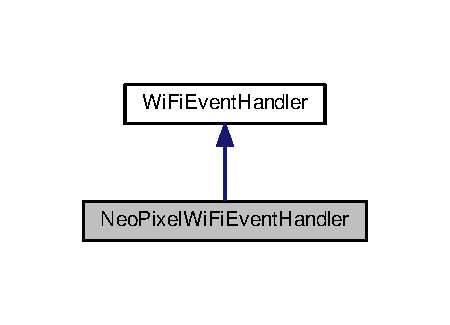
\includegraphics[width=216pt]{class_neo_pixel_wi_fi_event_handler__inherit__graph}
\end{center}
\end{figure}


Collaboration diagram for Neo\+Pixel\+Wi\+Fi\+Event\+Handler\+:\nopagebreak
\begin{figure}[H]
\begin{center}
\leavevmode
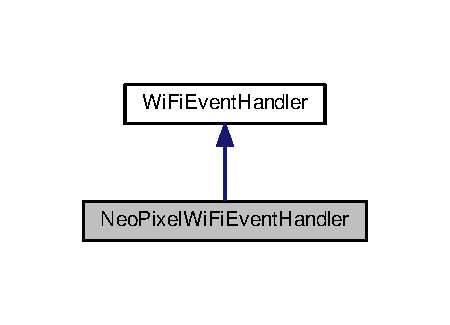
\includegraphics[width=216pt]{class_neo_pixel_wi_fi_event_handler__coll__graph}
\end{center}
\end{figure}
\subsection*{Public Member Functions}
\begin{DoxyCompactItemize}
\item 
{\bfseries Neo\+Pixel\+Wi\+Fi\+Event\+Handler} (gpio\+\_\+num\+\_\+t gpio\+Pin)\hypertarget{class_neo_pixel_wi_fi_event_handler_a821464c5875f6551f21108c613559022}{}\label{class_neo_pixel_wi_fi_event_handler_a821464c5875f6551f21108c613559022}

\item 
esp\+\_\+err\+\_\+t {\bfseries ap\+Start} () override\hypertarget{class_neo_pixel_wi_fi_event_handler_a0fac3188d6fc34c614e6ba60e8b06b8e}{}\label{class_neo_pixel_wi_fi_event_handler_a0fac3188d6fc34c614e6ba60e8b06b8e}

\item 
esp\+\_\+err\+\_\+t {\bfseries sta\+Connected} () override\hypertarget{class_neo_pixel_wi_fi_event_handler_ad7cdba5def110a1d1af2e4b82c6b9c06}{}\label{class_neo_pixel_wi_fi_event_handler_ad7cdba5def110a1d1af2e4b82c6b9c06}

\item 
esp\+\_\+err\+\_\+t \hyperlink{class_neo_pixel_wi_fi_event_handler_a3e9dffc7ccc2fab6e202695e53e3283a}{sta\+Got\+Ip} (system\+\_\+event\+\_\+sta\+\_\+got\+\_\+ip\+\_\+t event\+\_\+sta\+\_\+got\+\_\+ip) override
\item 
esp\+\_\+err\+\_\+t {\bfseries sta\+Disconnected} () override\hypertarget{class_neo_pixel_wi_fi_event_handler_a5de1c8ee6259a4963f28283244f434ca}{}\label{class_neo_pixel_wi_fi_event_handler_a5de1c8ee6259a4963f28283244f434ca}

\item 
esp\+\_\+err\+\_\+t {\bfseries wifi\+Ready} () override\hypertarget{class_neo_pixel_wi_fi_event_handler_a38e6ae3aed1d5a777c756a859a055676}{}\label{class_neo_pixel_wi_fi_event_handler_a38e6ae3aed1d5a777c756a859a055676}

\item 
esp\+\_\+err\+\_\+t {\bfseries sta\+Start} () override\hypertarget{class_neo_pixel_wi_fi_event_handler_a6961359273cba39f9e2c979746dfd57f}{}\label{class_neo_pixel_wi_fi_event_handler_a6961359273cba39f9e2c979746dfd57f}

\end{DoxyCompactItemize}


\subsection{Detailed Description}
Color a neopixel as a function of the Wi\+Fi state. 

When an E\+S\+P32 runs, we can\textquotesingle{}t tell by looking at it the state of the Wi\+Fi connection. This class provides a Wi\+Fi event handler that colors a Neo\+Pixel as a function of the state of the Wi\+Fi. 

\subsection{Member Function Documentation}
\index{Neo\+Pixel\+Wi\+Fi\+Event\+Handler@{Neo\+Pixel\+Wi\+Fi\+Event\+Handler}!sta\+Got\+Ip@{sta\+Got\+Ip}}
\index{sta\+Got\+Ip@{sta\+Got\+Ip}!Neo\+Pixel\+Wi\+Fi\+Event\+Handler@{Neo\+Pixel\+Wi\+Fi\+Event\+Handler}}
\subsubsection[{\texorpdfstring{sta\+Got\+Ip(system\+\_\+event\+\_\+sta\+\_\+got\+\_\+ip\+\_\+t event\+\_\+sta\+\_\+got\+\_\+ip) override}{staGotIp(system_event_sta_got_ip_t event_sta_got_ip) override}}]{\setlength{\rightskip}{0pt plus 5cm}esp\+\_\+err\+\_\+t Neo\+Pixel\+Wi\+Fi\+Event\+Handler\+::sta\+Got\+Ip (
\begin{DoxyParamCaption}
\item[{system\+\_\+event\+\_\+sta\+\_\+got\+\_\+ip\+\_\+t}]{event\+\_\+sta\+\_\+got\+\_\+ip}
\end{DoxyParamCaption}
)\hspace{0.3cm}{\ttfamily [override]}, {\ttfamily [virtual]}}\hypertarget{class_neo_pixel_wi_fi_event_handler_a3e9dffc7ccc2fab6e202695e53e3283a}{}\label{class_neo_pixel_wi_fi_event_handler_a3e9dffc7ccc2fab6e202695e53e3283a}
Handle having received/assigned an IP address when we are a station. \begin{DoxyReturn}{Returns}
An indication of whether or not we processed the event successfully. 
\end{DoxyReturn}


Reimplemented from \hyperlink{class_wi_fi_event_handler_ab01ad1cdc445bb2107125ec89a71886d}{Wi\+Fi\+Event\+Handler}.



The documentation for this class was generated from the following files\+:\begin{DoxyCompactItemize}
\item 
Neo\+Pixel\+Wi\+Fi\+Event\+Handler.\+h\item 
Neo\+Pixel\+Wi\+Fi\+Event\+Handler.\+cpp\end{DoxyCompactItemize}

\hypertarget{class_p_c_f8574}{}\section{P\+C\+F8574 Class Reference}
\label{class_p_c_f8574}\index{P\+C\+F8574@{P\+C\+F8574}}


Encapsulate a P\+C\+F8574 device.  




{\ttfamily \#include $<$P\+C\+F8574.\+h$>$}

\subsection*{Public Member Functions}
\begin{DoxyCompactItemize}
\item 
\hyperlink{class_p_c_f8574_aeaba161d7932ea2aa7f3bb9d05d36fba}{P\+C\+F8574} (int address)
\begin{DoxyCompactList}\small\item\em Class constructor. \end{DoxyCompactList}\item 
virtual \hyperlink{class_p_c_f8574_a20ddebfc28ba46646ca84f8c75034b34}{$\sim$\+P\+C\+F8574} ()\hypertarget{class_p_c_f8574_a20ddebfc28ba46646ca84f8c75034b34}{}\label{class_p_c_f8574_a20ddebfc28ba46646ca84f8c75034b34}

\begin{DoxyCompactList}\small\item\em Class instance destructor. \end{DoxyCompactList}\item 
void \hyperlink{class_p_c_f8574_abfe627fd97523863fa0075422b0158b6}{init} (gpio\+\_\+num\+\_\+t sda\+Pin=I2\+C\+::\+D\+E\+F\+A\+U\+L\+T\+\_\+\+S\+D\+A\+\_\+\+P\+IN, gpio\+\_\+num\+\_\+t clk\+Pin=I2\+C\+::\+D\+E\+F\+A\+U\+L\+T\+\_\+\+C\+L\+K\+\_\+\+P\+IN)
\begin{DoxyCompactList}\small\item\em Initialize the \hyperlink{class_p_c_f8574}{P\+C\+F8574} device. \end{DoxyCompactList}\item 
uint8\+\_\+t \hyperlink{class_p_c_f8574_a90a8a8c48e0530c7371dacabc1f6a282}{read} ()
\begin{DoxyCompactList}\small\item\em Read all the input bits from the device. \end{DoxyCompactList}\item 
bool \hyperlink{class_p_c_f8574_a4e484981cdf6451bb36a13f9d3a60400}{read\+Bit} (uint8\+\_\+t bit)
\begin{DoxyCompactList}\small\item\em Read the logic level on a given pin. \end{DoxyCompactList}\item 
void \hyperlink{class_p_c_f8574_a9663079a19f252a5edc2471f384bc28b}{set\+Invert} (bool value)
\begin{DoxyCompactList}\small\item\em Invert the bit values. Normally setting a pin\textquotesingle{}s value to 1 means that a high signal is generated and a 0 means a low signal is generated. Setting the inversion to true, inverts that meaning. \end{DoxyCompactList}\item 
void \hyperlink{class_p_c_f8574_a5d51dcc9e396c431561b8a0b044a9e6b}{write} (uint8\+\_\+t value)
\begin{DoxyCompactList}\small\item\em Set the output values of the device. \end{DoxyCompactList}\item 
void \hyperlink{class_p_c_f8574_a0d2f2b79548651b4fc40faefdc7156b0}{write\+Bit} (uint8\+\_\+t bit, bool value)
\begin{DoxyCompactList}\small\item\em Change the output value of a specific pin. \end{DoxyCompactList}\end{DoxyCompactItemize}


\subsection{Detailed Description}
Encapsulate a P\+C\+F8574 device. 

The P\+C\+F8574 is a 8 bit G\+P\+IO expander attached to I2C. It can read and write 8 bits of data and hence has 8 pins that can be used for input or output.

\begin{DoxySeeAlso}{See also}
\href{http://www.ti.com/product/PCF8574}{\tt P\+C\+F8574 home page} 
\end{DoxySeeAlso}


\subsection{Constructor \& Destructor Documentation}
\index{P\+C\+F8574@{P\+C\+F8574}!P\+C\+F8574@{P\+C\+F8574}}
\index{P\+C\+F8574@{P\+C\+F8574}!P\+C\+F8574@{P\+C\+F8574}}
\subsubsection[{\texorpdfstring{P\+C\+F8574(int address)}{PCF8574(int address)}}]{\setlength{\rightskip}{0pt plus 5cm}P\+C\+F8574\+::\+P\+C\+F8574 (
\begin{DoxyParamCaption}
\item[{int}]{address}
\end{DoxyParamCaption}
)}\hypertarget{class_p_c_f8574_aeaba161d7932ea2aa7f3bb9d05d36fba}{}\label{class_p_c_f8574_aeaba161d7932ea2aa7f3bb9d05d36fba}


Class constructor. 

The address is the address of the device on the I2C bus. This is the value 0x20 plus the value of the device input pins {\ttfamily A0}, {\ttfamily A1} and {\ttfamily A2}. This means that the address should be between 0x20 and 0x27.


\begin{DoxyParams}[1]{Parameters}
\mbox{\tt in}  & {\em address} & The I2C address of the device on the I2C bus. \\
\hline
\end{DoxyParams}


\subsection{Member Function Documentation}
\index{P\+C\+F8574@{P\+C\+F8574}!init@{init}}
\index{init@{init}!P\+C\+F8574@{P\+C\+F8574}}
\subsubsection[{\texorpdfstring{init(gpio\+\_\+num\+\_\+t sda\+Pin=\+I2\+C\+::\+D\+E\+F\+A\+U\+L\+T\+\_\+\+S\+D\+A\+\_\+\+P\+I\+N, gpio\+\_\+num\+\_\+t clk\+Pin=\+I2\+C\+::\+D\+E\+F\+A\+U\+L\+T\+\_\+\+C\+L\+K\+\_\+\+P\+I\+N)}{init(gpio_num_t sdaPin=I2C::DEFAULT_SDA_PIN, gpio_num_t clkPin=I2C::DEFAULT_CLK_PIN)}}]{\setlength{\rightskip}{0pt plus 5cm}void P\+C\+F8574\+::init (
\begin{DoxyParamCaption}
\item[{gpio\+\_\+num\+\_\+t}]{sda\+Pin = {\ttfamily I2C\+:\+:DEFAULT\+\_\+SDA\+\_\+PIN}, }
\item[{gpio\+\_\+num\+\_\+t}]{clk\+Pin = {\ttfamily I2C\+:\+:DEFAULT\+\_\+CLK\+\_\+PIN}}
\end{DoxyParamCaption}
)}\hypertarget{class_p_c_f8574_abfe627fd97523863fa0075422b0158b6}{}\label{class_p_c_f8574_abfe627fd97523863fa0075422b0158b6}


Initialize the \hyperlink{class_p_c_f8574}{P\+C\+F8574} device. 


\begin{DoxyParams}[1]{Parameters}
\mbox{\tt in}  & {\em sda\+Pin} & The pin to use for the I2C S\+DA functions. \\
\hline
\mbox{\tt in}  & {\em clk\+Pin} & The pin to use for the I2C C\+LK functions. \\
\hline
\end{DoxyParams}
\index{P\+C\+F8574@{P\+C\+F8574}!read@{read}}
\index{read@{read}!P\+C\+F8574@{P\+C\+F8574}}
\subsubsection[{\texorpdfstring{read()}{read()}}]{\setlength{\rightskip}{0pt plus 5cm}uint8\+\_\+t P\+C\+F8574\+::read (
\begin{DoxyParamCaption}
{}
\end{DoxyParamCaption}
)}\hypertarget{class_p_c_f8574_a90a8a8c48e0530c7371dacabc1f6a282}{}\label{class_p_c_f8574_a90a8a8c48e0530c7371dacabc1f6a282}


Read all the input bits from the device. 

\begin{DoxyReturn}{Returns}
An 8 bit value representing the values on each of the input pins. 
\end{DoxyReturn}
\index{P\+C\+F8574@{P\+C\+F8574}!read\+Bit@{read\+Bit}}
\index{read\+Bit@{read\+Bit}!P\+C\+F8574@{P\+C\+F8574}}
\subsubsection[{\texorpdfstring{read\+Bit(uint8\+\_\+t bit)}{readBit(uint8_t bit)}}]{\setlength{\rightskip}{0pt plus 5cm}bool P\+C\+F8574\+::read\+Bit (
\begin{DoxyParamCaption}
\item[{uint8\+\_\+t}]{bit}
\end{DoxyParamCaption}
)}\hypertarget{class_p_c_f8574_a4e484981cdf6451bb36a13f9d3a60400}{}\label{class_p_c_f8574_a4e484981cdf6451bb36a13f9d3a60400}


Read the logic level on a given pin. 


\begin{DoxyParams}[1]{Parameters}
\mbox{\tt in}  & {\em bit} & The input pin of the device to read. Values are 0-\/7. \\
\hline
\end{DoxyParams}
\begin{DoxyReturn}{Returns}
True if the pin is high, false otherwise. Undefined if there is no signal on the pin. 
\end{DoxyReturn}
\index{P\+C\+F8574@{P\+C\+F8574}!set\+Invert@{set\+Invert}}
\index{set\+Invert@{set\+Invert}!P\+C\+F8574@{P\+C\+F8574}}
\subsubsection[{\texorpdfstring{set\+Invert(bool value)}{setInvert(bool value)}}]{\setlength{\rightskip}{0pt plus 5cm}void P\+C\+F8574\+::set\+Invert (
\begin{DoxyParamCaption}
\item[{bool}]{value}
\end{DoxyParamCaption}
)}\hypertarget{class_p_c_f8574_a9663079a19f252a5edc2471f384bc28b}{}\label{class_p_c_f8574_a9663079a19f252a5edc2471f384bc28b}


Invert the bit values. Normally setting a pin\textquotesingle{}s value to 1 means that a high signal is generated and a 0 means a low signal is generated. Setting the inversion to true, inverts that meaning. 


\begin{DoxyParams}[1]{Parameters}
\mbox{\tt in}  & {\em value} & True if we wish to invert the signals and false otherwise. \\
\hline
\end{DoxyParams}
\index{P\+C\+F8574@{P\+C\+F8574}!write@{write}}
\index{write@{write}!P\+C\+F8574@{P\+C\+F8574}}
\subsubsection[{\texorpdfstring{write(uint8\+\_\+t value)}{write(uint8_t value)}}]{\setlength{\rightskip}{0pt plus 5cm}void P\+C\+F8574\+::write (
\begin{DoxyParamCaption}
\item[{uint8\+\_\+t}]{value}
\end{DoxyParamCaption}
)}\hypertarget{class_p_c_f8574_a5d51dcc9e396c431561b8a0b044a9e6b}{}\label{class_p_c_f8574_a5d51dcc9e396c431561b8a0b044a9e6b}


Set the output values of the device. 


\begin{DoxyParams}[1]{Parameters}
\mbox{\tt in}  & {\em value} & The bit pattern to set on the output. \\
\hline
\end{DoxyParams}
\index{P\+C\+F8574@{P\+C\+F8574}!write\+Bit@{write\+Bit}}
\index{write\+Bit@{write\+Bit}!P\+C\+F8574@{P\+C\+F8574}}
\subsubsection[{\texorpdfstring{write\+Bit(uint8\+\_\+t bit, bool value)}{writeBit(uint8_t bit, bool value)}}]{\setlength{\rightskip}{0pt plus 5cm}void P\+C\+F8574\+::write\+Bit (
\begin{DoxyParamCaption}
\item[{uint8\+\_\+t}]{bit, }
\item[{bool}]{value}
\end{DoxyParamCaption}
)}\hypertarget{class_p_c_f8574_a0d2f2b79548651b4fc40faefdc7156b0}{}\label{class_p_c_f8574_a0d2f2b79548651b4fc40faefdc7156b0}


Change the output value of a specific pin. 

The other bits beyond the one setting retain their values from the previous call to \hyperlink{class_p_c_f8574_a5d51dcc9e396c431561b8a0b044a9e6b}{write()} or previous calls to \hyperlink{class_p_c_f8574_a0d2f2b79548651b4fc40faefdc7156b0}{write\+Bit()}.


\begin{DoxyParams}[1]{Parameters}
\mbox{\tt in}  & {\em bit} & The pin to have its value changed. The pin may be 0-\/7. \\
\hline
\mbox{\tt in}  & {\em value} & The logic level to appear on the identified output pin. \\
\hline
\end{DoxyParams}


The documentation for this class was generated from the following files\+:\begin{DoxyCompactItemize}
\item 
P\+C\+F8574.\+h\item 
P\+C\+F8574.\+cpp\end{DoxyCompactItemize}

\hypertarget{structpixel__t}{}\section{pixel\+\_\+t Struct Reference}
\label{structpixel__t}\index{pixel\+\_\+t@{pixel\+\_\+t}}


A data type representing the color of a pixel.  




{\ttfamily \#include $<$W\+S2812.\+h$>$}

\subsection*{Public Attributes}
\begin{DoxyCompactItemize}
\item 
uint8\+\_\+t {\bfseries red}\hypertarget{structpixel__t_a912496dc782ecc3cea2f89eb79b7c9a0}{}\label{structpixel__t_a912496dc782ecc3cea2f89eb79b7c9a0}

\item 
uint8\+\_\+t {\bfseries green}\hypertarget{structpixel__t_a945c55299b107661d118e849b388039b}{}\label{structpixel__t_a945c55299b107661d118e849b388039b}

\item 
uint8\+\_\+t {\bfseries blue}\hypertarget{structpixel__t_a32f72c7c5c7c932c7e554d05f7390941}{}\label{structpixel__t_a32f72c7c5c7c932c7e554d05f7390941}

\end{DoxyCompactItemize}


\subsection{Detailed Description}
A data type representing the color of a pixel. 

The documentation for this struct was generated from the following file\+:\begin{DoxyCompactItemize}
\item 
W\+S2812.\+h\end{DoxyCompactItemize}

\hypertarget{class_p_w_m}{}\section{P\+WM Class Reference}
\label{class_p_w_m}\index{P\+WM@{P\+WM}}


A wrapper for E\+S\+P32 P\+WM control.  




{\ttfamily \#include $<$P\+W\+M.\+h$>$}

\subsection*{Public Member Functions}
\begin{DoxyCompactItemize}
\item 
\hyperlink{class_p_w_m_ad2d67d2ed4c65173889a7528ff4d2fa4}{P\+WM} (ledc\+\_\+timer\+\_\+bit\+\_\+t bit\+Size, ledc\+\_\+timer\+\_\+t timer, ledc\+\_\+channel\+\_\+t channel, int gpio\+Num)
\begin{DoxyCompactList}\small\item\em Construct an instance. \end{DoxyCompactList}\item 
uint32\+\_\+t \hyperlink{class_p_w_m_a7d6403597b936f73be3a53b330d15f52}{get\+Duty} ()
\begin{DoxyCompactList}\small\item\em Get the duty cycle value. \end{DoxyCompactList}\item 
uint32\+\_\+t \hyperlink{class_p_w_m_a70e2e1ad7736f241eef020ec4c7e7fff}{get\+Frequency} ()
\begin{DoxyCompactList}\small\item\em Get the frequency/period in Hz. \end{DoxyCompactList}\item 
void \hyperlink{class_p_w_m_adae9be9a8c34c42d0f81dd0b4a24c14f}{set\+Duty} (uint32\+\_\+t duty)\hypertarget{class_p_w_m_adae9be9a8c34c42d0f81dd0b4a24c14f}{}\label{class_p_w_m_adae9be9a8c34c42d0f81dd0b4a24c14f}

\begin{DoxyCompactList}\small\item\em Set the duty cycle value. \end{DoxyCompactList}\item 
void \hyperlink{class_p_w_m_a51543c5bf29d9f3ae83c7f5af176895d}{set\+Frequency} (uint32\+\_\+t freq)\hypertarget{class_p_w_m_a51543c5bf29d9f3ae83c7f5af176895d}{}\label{class_p_w_m_a51543c5bf29d9f3ae83c7f5af176895d}

\begin{DoxyCompactList}\small\item\em Set the frequency/period in Hz. \end{DoxyCompactList}\item 
void \hyperlink{class_p_w_m_a839027de87bbee57a3dabe21d254d892}{stop} (bool idle\+Level=false)\hypertarget{class_p_w_m_a839027de87bbee57a3dabe21d254d892}{}\label{class_p_w_m_a839027de87bbee57a3dabe21d254d892}

\begin{DoxyCompactList}\small\item\em Stop the P\+WM. \end{DoxyCompactList}\end{DoxyCompactItemize}


\subsection{Detailed Description}
A wrapper for E\+S\+P32 P\+WM control. 

\subsection{Constructor \& Destructor Documentation}
\index{P\+WM@{P\+WM}!P\+WM@{P\+WM}}
\index{P\+WM@{P\+WM}!P\+WM@{P\+WM}}
\subsubsection[{\texorpdfstring{P\+W\+M(ledc\+\_\+timer\+\_\+bit\+\_\+t bit\+Size, ledc\+\_\+timer\+\_\+t timer, ledc\+\_\+channel\+\_\+t channel, int gpio\+Num)}{PWM(ledc_timer_bit_t bitSize, ledc_timer_t timer, ledc_channel_t channel, int gpioNum)}}]{\setlength{\rightskip}{0pt plus 5cm}P\+W\+M\+::\+P\+WM (
\begin{DoxyParamCaption}
\item[{ledc\+\_\+timer\+\_\+bit\+\_\+t}]{bit\+Size, }
\item[{ledc\+\_\+timer\+\_\+t}]{timer, }
\item[{ledc\+\_\+channel\+\_\+t}]{channel, }
\item[{int}]{gpio\+Num}
\end{DoxyParamCaption}
)}\hypertarget{class_p_w_m_ad2d67d2ed4c65173889a7528ff4d2fa4}{}\label{class_p_w_m_ad2d67d2ed4c65173889a7528ff4d2fa4}


Construct an instance. 


\begin{DoxyParams}[1]{Parameters}
\mbox{\tt in}  & {\em bit\+Size} & The size in bits of the timer. Allowed values are L\+E\+D\+C\+\_\+\+T\+I\+M\+E\+R\+\_\+10\+\_\+\+B\+IT, L\+E\+D\+C\+\_\+\+T\+I\+M\+E\+R\+\_\+11\+\_\+\+B\+IT, L\+E\+D\+C\+\_\+\+T\+I\+M\+E\+R\+\_\+12\+\_\+\+B\+IT, L\+E\+D\+C\+\_\+\+T\+I\+M\+E\+R\+\_\+13\+\_\+\+B\+IT, L\+E\+D\+C\+\_\+\+T\+I\+M\+E\+R\+\_\+14\+\_\+\+B\+IT, L\+E\+D\+C\+\_\+\+T\+I\+M\+E\+R\+\_\+15\+\_\+\+B\+IT. \\
\hline
\mbox{\tt in}  & {\em timer} & The timer to use. A value of L\+E\+D\+C\+\_\+\+T\+I\+M\+E\+R0, L\+E\+D\+C\+\_\+\+T\+I\+M\+E\+R1, L\+E\+D\+C\+\_\+\+T\+I\+M\+E\+R2 or L\+E\+D\+C\+\_\+\+T\+I\+M\+E\+R3. \\
\hline
\mbox{\tt in}  & {\em channel} & The channel to use. A value from L\+E\+D\+C\+\_\+\+C\+H\+A\+N\+N\+E\+L0 to L\+E\+D\+C\+\_\+\+C\+H\+A\+N\+N\+E\+L1. \\
\hline
\end{DoxyParams}


\subsection{Member Function Documentation}
\index{P\+WM@{P\+WM}!get\+Duty@{get\+Duty}}
\index{get\+Duty@{get\+Duty}!P\+WM@{P\+WM}}
\subsubsection[{\texorpdfstring{get\+Duty()}{getDuty()}}]{\setlength{\rightskip}{0pt plus 5cm}uint32\+\_\+t P\+W\+M\+::get\+Duty (
\begin{DoxyParamCaption}
{}
\end{DoxyParamCaption}
)}\hypertarget{class_p_w_m_a7d6403597b936f73be3a53b330d15f52}{}\label{class_p_w_m_a7d6403597b936f73be3a53b330d15f52}


Get the duty cycle value. 

\begin{DoxyReturn}{Returns}
The duty cycle value. 
\end{DoxyReturn}
\index{P\+WM@{P\+WM}!get\+Frequency@{get\+Frequency}}
\index{get\+Frequency@{get\+Frequency}!P\+WM@{P\+WM}}
\subsubsection[{\texorpdfstring{get\+Frequency()}{getFrequency()}}]{\setlength{\rightskip}{0pt plus 5cm}uint32\+\_\+t P\+W\+M\+::get\+Frequency (
\begin{DoxyParamCaption}
{}
\end{DoxyParamCaption}
)}\hypertarget{class_p_w_m_a70e2e1ad7736f241eef020ec4c7e7fff}{}\label{class_p_w_m_a70e2e1ad7736f241eef020ec4c7e7fff}


Get the frequency/period in Hz. 

\begin{DoxyReturn}{Returns}
The frequency/period in Hz. 
\end{DoxyReturn}


The documentation for this class was generated from the following files\+:\begin{DoxyCompactItemize}
\item 
P\+W\+M.\+h\item 
P\+W\+M.\+cpp\end{DoxyCompactItemize}

\hypertarget{class_r_e_s_t_client}{}\section{R\+E\+S\+T\+Client Class Reference}
\label{class_r_e_s_t_client}\index{R\+E\+S\+T\+Client@{R\+E\+S\+T\+Client}}


Encapsulate a R\+E\+ST client call.  




{\ttfamily \#include $<$R\+E\+S\+T\+Client.\+h$>$}

\subsection*{Public Member Functions}
\begin{DoxyCompactItemize}
\item 
void \hyperlink{class_r_e_s_t_client_a3b60574f73a5beb9fef7253f9bdf35d5}{add\+Header} (std\+::string name, std\+::string value)
\begin{DoxyCompactList}\small\item\em Add a header to the list of headers. \end{DoxyCompactList}\item 
void \hyperlink{class_r_e_s_t_client_ad49cc3c5eae7060f20ab01b673ca798d}{get} ()\hypertarget{class_r_e_s_t_client_ad49cc3c5eae7060f20ab01b673ca798d}{}\label{class_r_e_s_t_client_ad49cc3c5eae7060f20ab01b673ca798d}

\begin{DoxyCompactList}\small\item\em Perform an H\+T\+TP G\+ET request. \end{DoxyCompactList}\item 
std\+::string \hyperlink{class_r_e_s_t_client_ad064323ad773353724ce654c449b0ce5}{get\+Error\+Message} ()\hypertarget{class_r_e_s_t_client_ad064323ad773353724ce654c449b0ce5}{}\label{class_r_e_s_t_client_ad064323ad773353724ce654c449b0ce5}

\begin{DoxyCompactList}\small\item\em Get the last error message. \end{DoxyCompactList}\item 
std\+::string {\bfseries get\+Response} ()\hypertarget{class_r_e_s_t_client_adfad79ecfa8e27972b3fb545a6c04c26}{}\label{class_r_e_s_t_client_adfad79ecfa8e27972b3fb545a6c04c26}

\item 
\hyperlink{class_r_e_s_t_timings}{R\+E\+S\+T\+Timings} $\ast$ {\bfseries get\+Timings} ()\hypertarget{class_r_e_s_t_client_a43e5aafd08ec94a3d338078661a8c48d}{}\label{class_r_e_s_t_client_a43e5aafd08ec94a3d338078661a8c48d}

\item 
void \hyperlink{class_r_e_s_t_client_ac9f65761dbc3dcac5b2b46c628873414}{post} (std\+::string body)
\begin{DoxyCompactList}\small\item\em Perform an H\+T\+TP P\+O\+ST request. \end{DoxyCompactList}\item 
void \hyperlink{class_r_e_s_t_client_aafaf9da1d856e92c7c44e4d089257557}{set\+U\+RL} (std\+::string url)
\begin{DoxyCompactList}\small\item\em Set the U\+RL for the target. \end{DoxyCompactList}\item 
void \hyperlink{class_r_e_s_t_client_a2f5f4b033dfa6d2c6746221ff32a5fb5}{set\+Verbose} (bool value)
\begin{DoxyCompactList}\small\item\em Set the verbosity flag. \end{DoxyCompactList}\end{DoxyCompactItemize}
\subsection*{Friends}
\begin{DoxyCompactItemize}
\item 
class {\bfseries R\+E\+S\+T\+Timings}\hypertarget{class_r_e_s_t_client_a3dc2262849e3935cec7f09790a169ae5}{}\label{class_r_e_s_t_client_a3dc2262849e3935cec7f09790a169ae5}

\end{DoxyCompactItemize}


\subsection{Detailed Description}
Encapsulate a R\+E\+ST client call. 

\subsection{Member Function Documentation}
\index{R\+E\+S\+T\+Client@{R\+E\+S\+T\+Client}!add\+Header@{add\+Header}}
\index{add\+Header@{add\+Header}!R\+E\+S\+T\+Client@{R\+E\+S\+T\+Client}}
\subsubsection[{\texorpdfstring{add\+Header(std\+::string name, std\+::string value)}{addHeader(std::string name, std::string value)}}]{\setlength{\rightskip}{0pt plus 5cm}void R\+E\+S\+T\+Client\+::add\+Header (
\begin{DoxyParamCaption}
\item[{std\+::string}]{name, }
\item[{std\+::string}]{value}
\end{DoxyParamCaption}
)}\hypertarget{class_r_e_s_t_client_a3b60574f73a5beb9fef7253f9bdf35d5}{}\label{class_r_e_s_t_client_a3b60574f73a5beb9fef7253f9bdf35d5}


Add a header to the list of headers. 

For example\+:


\begin{DoxyCode}
client.addHeader(\textcolor{stringliteral}{"Content-Type"}, \textcolor{stringliteral}{"application/json"});
\end{DoxyCode}



\begin{DoxyParams}[1]{Parameters}
\mbox{\tt in}  & {\em name} & The name of the header to be added. \\
\hline
\mbox{\tt in}  & {\em value} & The value of the header to be added. \\
\hline
\end{DoxyParams}
\index{R\+E\+S\+T\+Client@{R\+E\+S\+T\+Client}!post@{post}}
\index{post@{post}!R\+E\+S\+T\+Client@{R\+E\+S\+T\+Client}}
\subsubsection[{\texorpdfstring{post(std\+::string body)}{post(std::string body)}}]{\setlength{\rightskip}{0pt plus 5cm}void R\+E\+S\+T\+Client\+::post (
\begin{DoxyParamCaption}
\item[{std\+::string}]{body}
\end{DoxyParamCaption}
)}\hypertarget{class_r_e_s_t_client_ac9f65761dbc3dcac5b2b46c628873414}{}\label{class_r_e_s_t_client_ac9f65761dbc3dcac5b2b46c628873414}


Perform an H\+T\+TP P\+O\+ST request. 


\begin{DoxyParams}[1]{Parameters}
\mbox{\tt in}  & {\em body} & The body of the payload to send with the post request. \\
\hline
\end{DoxyParams}
\index{R\+E\+S\+T\+Client@{R\+E\+S\+T\+Client}!set\+U\+RL@{set\+U\+RL}}
\index{set\+U\+RL@{set\+U\+RL}!R\+E\+S\+T\+Client@{R\+E\+S\+T\+Client}}
\subsubsection[{\texorpdfstring{set\+U\+R\+L(std\+::string url)}{setURL(std::string url)}}]{\setlength{\rightskip}{0pt plus 5cm}void R\+E\+S\+T\+Client\+::set\+U\+RL (
\begin{DoxyParamCaption}
\item[{std\+::string}]{url}
\end{DoxyParamCaption}
)\hspace{0.3cm}{\ttfamily [inline]}}\hypertarget{class_r_e_s_t_client_aafaf9da1d856e92c7c44e4d089257557}{}\label{class_r_e_s_t_client_aafaf9da1d856e92c7c44e4d089257557}


Set the U\+RL for the target. 


\begin{DoxyParams}[1]{Parameters}
\mbox{\tt in}  & {\em url} & The target for H\+T\+TP request. \\
\hline
\end{DoxyParams}
\index{R\+E\+S\+T\+Client@{R\+E\+S\+T\+Client}!set\+Verbose@{set\+Verbose}}
\index{set\+Verbose@{set\+Verbose}!R\+E\+S\+T\+Client@{R\+E\+S\+T\+Client}}
\subsubsection[{\texorpdfstring{set\+Verbose(bool value)}{setVerbose(bool value)}}]{\setlength{\rightskip}{0pt plus 5cm}void R\+E\+S\+T\+Client\+::set\+Verbose (
\begin{DoxyParamCaption}
\item[{bool}]{value}
\end{DoxyParamCaption}
)\hspace{0.3cm}{\ttfamily [inline]}}\hypertarget{class_r_e_s_t_client_a2f5f4b033dfa6d2c6746221ff32a5fb5}{}\label{class_r_e_s_t_client_a2f5f4b033dfa6d2c6746221ff32a5fb5}


Set the verbosity flag. 


\begin{DoxyParams}[1]{Parameters}
\mbox{\tt in}  & {\em The} & value of the verbosity. \\
\hline
\end{DoxyParams}


The documentation for this class was generated from the following files\+:\begin{DoxyCompactItemize}
\item 
R\+E\+S\+T\+Client.\+h\item 
R\+E\+S\+T\+Client.\+cpp\end{DoxyCompactItemize}

\hypertarget{class_r_e_s_t_timings}{}\section{R\+E\+S\+T\+Timings Class Reference}
\label{class_r_e_s_t_timings}\index{R\+E\+S\+T\+Timings@{R\+E\+S\+T\+Timings}}


Timing data for R\+E\+ST calls.  




{\ttfamily \#include $<$R\+E\+S\+T\+Client.\+h$>$}

\subsection*{Public Member Functions}
\begin{DoxyCompactItemize}
\item 
{\bfseries R\+E\+S\+T\+Timings} (\hyperlink{class_r_e_s_t_client}{R\+E\+S\+T\+Client} $\ast$client)\hypertarget{class_r_e_s_t_timings_aee2e9a6dfca7cb179fd9a310c206b0b6}{}\label{class_r_e_s_t_timings_aee2e9a6dfca7cb179fd9a310c206b0b6}

\item 
void \hyperlink{class_r_e_s_t_timings_a567d407b236bfbfd848f82bc5d79bcd4}{refresh} ()\hypertarget{class_r_e_s_t_timings_a567d407b236bfbfd848f82bc5d79bcd4}{}\label{class_r_e_s_t_timings_a567d407b236bfbfd848f82bc5d79bcd4}

\begin{DoxyCompactList}\small\item\em Refresh the timings information. \end{DoxyCompactList}\item 
std\+::string \hyperlink{class_r_e_s_t_timings_a38883c6a6e99470292cbfa847db73830}{to\+String} ()
\begin{DoxyCompactList}\small\item\em Return the timings information as a string. \end{DoxyCompactList}\end{DoxyCompactItemize}


\subsection{Detailed Description}
Timing data for R\+E\+ST calls. 

\subsection{Member Function Documentation}
\index{R\+E\+S\+T\+Timings@{R\+E\+S\+T\+Timings}!to\+String@{to\+String}}
\index{to\+String@{to\+String}!R\+E\+S\+T\+Timings@{R\+E\+S\+T\+Timings}}
\subsubsection[{\texorpdfstring{to\+String()}{toString()}}]{\setlength{\rightskip}{0pt plus 5cm}std\+::string R\+E\+S\+T\+Timings\+::to\+String (
\begin{DoxyParamCaption}
{}
\end{DoxyParamCaption}
)}\hypertarget{class_r_e_s_t_timings_a38883c6a6e99470292cbfa847db73830}{}\label{class_r_e_s_t_timings_a38883c6a6e99470292cbfa847db73830}


Return the timings information as a string. 

\begin{DoxyReturn}{Returns}
The timings information. 
\end{DoxyReturn}


The documentation for this class was generated from the following files\+:\begin{DoxyCompactItemize}
\item 
R\+E\+S\+T\+Client.\+h\item 
R\+E\+S\+T\+Client.\+cpp\end{DoxyCompactItemize}

\hypertarget{class_r_m_t}{}\section{R\+MT Class Reference}
\label{class_r_m_t}\index{R\+MT@{R\+MT}}


Drive the \hyperlink{class_r_m_t}{R\+MT} peripheral.  




{\ttfamily \#include $<$R\+M\+T.\+h$>$}

\subsection*{Public Member Functions}
\begin{DoxyCompactItemize}
\item 
\hyperlink{class_r_m_t_ab4e0f3b8ff01d7604d0bc52bc44c590f}{R\+MT} (gpio\+\_\+num\+\_\+t pin, rmt\+\_\+channel\+\_\+t channel=R\+M\+T\+\_\+\+C\+H\+A\+N\+N\+E\+L\+\_\+0)
\begin{DoxyCompactList}\small\item\em Create a class instance. \end{DoxyCompactList}\item 
virtual \hyperlink{class_r_m_t_a5b59083a872122d19e34d5585a06914f}{$\sim$\+R\+MT} ()\hypertarget{class_r_m_t_a5b59083a872122d19e34d5585a06914f}{}\label{class_r_m_t_a5b59083a872122d19e34d5585a06914f}

\begin{DoxyCompactList}\small\item\em Class destructor. \end{DoxyCompactList}\item 
void \hyperlink{class_r_m_t_a29461fa2ff9900b5ddff5dd0ec35abb0}{add} (bool level, uint32\+\_\+t duration)
\begin{DoxyCompactList}\small\item\em Add a level/duration to the transaction to be written. \end{DoxyCompactList}\item 
void \hyperlink{class_r_m_t_acf727f6cdf9b357a320a19661f90e6c4}{clear} ()\hypertarget{class_r_m_t_acf727f6cdf9b357a320a19661f90e6c4}{}\label{class_r_m_t_acf727f6cdf9b357a320a19661f90e6c4}

\begin{DoxyCompactList}\small\item\em Clear any previously written level/duration pairs that have not been sent. \end{DoxyCompactList}\item 
void \hyperlink{class_r_m_t_af1b130bf271e12117511f75f6e08fcea}{rx\+Start} ()\hypertarget{class_r_m_t_af1b130bf271e12117511f75f6e08fcea}{}\label{class_r_m_t_af1b130bf271e12117511f75f6e08fcea}

\begin{DoxyCompactList}\small\item\em Start receiving. \end{DoxyCompactList}\item 
void \hyperlink{class_r_m_t_a0f3abda595084f39bc5a524b468feeab}{rx\+Stop} ()\hypertarget{class_r_m_t_a0f3abda595084f39bc5a524b468feeab}{}\label{class_r_m_t_a0f3abda595084f39bc5a524b468feeab}

\begin{DoxyCompactList}\small\item\em Stop receiving. \end{DoxyCompactList}\item 
void \hyperlink{class_r_m_t_a4dd6deb2c682661f70dd9b17519455e6}{tx\+Start} ()\hypertarget{class_r_m_t_a4dd6deb2c682661f70dd9b17519455e6}{}\label{class_r_m_t_a4dd6deb2c682661f70dd9b17519455e6}

\begin{DoxyCompactList}\small\item\em Start transmitting. \end{DoxyCompactList}\item 
void \hyperlink{class_r_m_t_a5b4184c0472608379fdd868e3aa68e15}{tx\+Stop} ()\hypertarget{class_r_m_t_a5b4184c0472608379fdd868e3aa68e15}{}\label{class_r_m_t_a5b4184c0472608379fdd868e3aa68e15}

\begin{DoxyCompactList}\small\item\em Stop transmitting. \end{DoxyCompactList}\item 
void \hyperlink{class_r_m_t_a0eef7f4df02df1f9e0f33cde2cb3ee1f}{write} ()
\begin{DoxyCompactList}\small\item\em Write the items out through the \hyperlink{class_r_m_t}{R\+MT}. \end{DoxyCompactList}\end{DoxyCompactItemize}


\subsection{Detailed Description}
Drive the \hyperlink{class_r_m_t}{R\+MT} peripheral. 

\subsection{Constructor \& Destructor Documentation}
\index{R\+MT@{R\+MT}!R\+MT@{R\+MT}}
\index{R\+MT@{R\+MT}!R\+MT@{R\+MT}}
\subsubsection[{\texorpdfstring{R\+M\+T(gpio\+\_\+num\+\_\+t pin, rmt\+\_\+channel\+\_\+t channel=\+R\+M\+T\+\_\+\+C\+H\+A\+N\+N\+E\+L\+\_\+0)}{RMT(gpio_num_t pin, rmt_channel_t channel=RMT_CHANNEL_0)}}]{\setlength{\rightskip}{0pt plus 5cm}R\+M\+T\+::\+R\+MT (
\begin{DoxyParamCaption}
\item[{gpio\+\_\+num\+\_\+t}]{pin, }
\item[{rmt\+\_\+channel\+\_\+t}]{channel = {\ttfamily RMT\+\_\+CHANNEL\+\_\+0}}
\end{DoxyParamCaption}
)}\hypertarget{class_r_m_t_ab4e0f3b8ff01d7604d0bc52bc44c590f}{}\label{class_r_m_t_ab4e0f3b8ff01d7604d0bc52bc44c590f}


Create a class instance. 


\begin{DoxyParams}[1]{Parameters}
\mbox{\tt in}  & {\em pin} & The \hyperlink{class_g_p_i_o}{G\+P\+IO} pin on which the signal is sent/received. \\
\hline
\mbox{\tt in}  & {\em channel} & The \hyperlink{class_r_m_t}{R\+MT} channel to work with. \\
\hline
\end{DoxyParams}


\subsection{Member Function Documentation}
\index{R\+MT@{R\+MT}!add@{add}}
\index{add@{add}!R\+MT@{R\+MT}}
\subsubsection[{\texorpdfstring{add(bool level, uint32\+\_\+t duration)}{add(bool level, uint32_t duration)}}]{\setlength{\rightskip}{0pt plus 5cm}void R\+M\+T\+::add (
\begin{DoxyParamCaption}
\item[{bool}]{level, }
\item[{uint32\+\_\+t}]{duration}
\end{DoxyParamCaption}
)}\hypertarget{class_r_m_t_a29461fa2ff9900b5ddff5dd0ec35abb0}{}\label{class_r_m_t_a29461fa2ff9900b5ddff5dd0ec35abb0}


Add a level/duration to the transaction to be written. 


\begin{DoxyParams}[1]{Parameters}
\mbox{\tt in}  & {\em level} & The level of the bit to output. \\
\hline
\mbox{\tt in}  & {\em duration} & The duration of the bit to output. \\
\hline
\end{DoxyParams}
\index{R\+MT@{R\+MT}!write@{write}}
\index{write@{write}!R\+MT@{R\+MT}}
\subsubsection[{\texorpdfstring{write()}{write()}}]{\setlength{\rightskip}{0pt plus 5cm}void R\+M\+T\+::write (
\begin{DoxyParamCaption}
{}
\end{DoxyParamCaption}
)}\hypertarget{class_r_m_t_a0eef7f4df02df1f9e0f33cde2cb3ee1f}{}\label{class_r_m_t_a0eef7f4df02df1f9e0f33cde2cb3ee1f}


Write the items out through the \hyperlink{class_r_m_t}{R\+MT}. 

The level/duration set of bits that were added to the transaction are written out through the \hyperlink{class_r_m_t}{R\+MT} device. After transmission, the list of level/durations is cleared. 

The documentation for this class was generated from the following files\+:\begin{DoxyCompactItemize}
\item 
R\+M\+T.\+h\item 
R\+M\+T.\+cpp\end{DoxyCompactItemize}

\hypertarget{class_socket}{}\section{Socket Class Reference}
\label{class_socket}\index{Socket@{Socket}}


Encapsulate a socket.  




{\ttfamily \#include $<$Socket.\+h$>$}

\subsection*{Public Member Functions}
\begin{DoxyCompactItemize}
\item 
void {\bfseries close\+\_\+cpp} ()\hypertarget{class_socket_a2f39e65b68fcae82a3c9f2665c7ab812}{}\label{class_socket_a2f39e65b68fcae82a3c9f2665c7ab812}

\item 
int \hyperlink{class_socket_a453f3704a57418550aa4f93eb3e7e583}{connect\+\_\+cpp} (struct in\+\_\+addr address, uint16\+\_\+t port)
\begin{DoxyCompactList}\small\item\em Connect to a partner. \end{DoxyCompactList}\item 
int \hyperlink{class_socket_a67d57f2841b0469f8d5e4d1c73e81871}{connect\+\_\+cpp} (char $\ast$address, uint16\+\_\+t port)
\begin{DoxyCompactList}\small\item\em Connect to a partner. \end{DoxyCompactList}\item 
int \hyperlink{class_socket_a58b0eba9803e12930dff91eabe00ae18}{receive\+\_\+cpp} (uint8\+\_\+t $\ast$data, size\+\_\+t length)
\begin{DoxyCompactList}\small\item\em Receive data from the partner. \end{DoxyCompactList}\item 
void \hyperlink{class_socket_a75d4cde966c827df816de5c086dde520}{send\+\_\+cpp} (const uint8\+\_\+t $\ast$data, size\+\_\+t length)
\begin{DoxyCompactList}\small\item\em Send data to the partner. \end{DoxyCompactList}\item 
void \hyperlink{class_socket_acfe9059df34833daa92b381492e20446}{send\+\_\+cpp} (std\+::string value)
\begin{DoxyCompactList}\small\item\em Send a string to the partner. \end{DoxyCompactList}\end{DoxyCompactItemize}


\subsection{Detailed Description}
Encapsulate a socket. 

Using this class we can connect to a partner T\+CP server. Once connected, we can perform send and receive requests to send and receive data. We should not attempt to send or receive until after a successful connect nor should we send or receive after closing the socket. 

\subsection{Member Function Documentation}
\index{Socket@{Socket}!connect\+\_\+cpp@{connect\+\_\+cpp}}
\index{connect\+\_\+cpp@{connect\+\_\+cpp}!Socket@{Socket}}
\subsubsection[{\texorpdfstring{connect\+\_\+cpp(struct in\+\_\+addr address, uint16\+\_\+t port)}{connect_cpp(struct in_addr address, uint16_t port)}}]{\setlength{\rightskip}{0pt plus 5cm}int Socket\+::connect\+\_\+cpp (
\begin{DoxyParamCaption}
\item[{struct in\+\_\+addr}]{address, }
\item[{uint16\+\_\+t}]{port}
\end{DoxyParamCaption}
)}\hypertarget{class_socket_a453f3704a57418550aa4f93eb3e7e583}{}\label{class_socket_a453f3704a57418550aa4f93eb3e7e583}


Connect to a partner. 


\begin{DoxyParams}[1]{Parameters}
\mbox{\tt in}  & {\em address} & The IP address of the partner. \\
\hline
\mbox{\tt in}  & {\em port} & The port number of the partner. \\
\hline
\end{DoxyParams}
\begin{DoxyReturn}{Returns}
Success or failure of the connection. 
\end{DoxyReturn}
\index{Socket@{Socket}!connect\+\_\+cpp@{connect\+\_\+cpp}}
\index{connect\+\_\+cpp@{connect\+\_\+cpp}!Socket@{Socket}}
\subsubsection[{\texorpdfstring{connect\+\_\+cpp(char $\ast$address, uint16\+\_\+t port)}{connect_cpp(char *address, uint16_t port)}}]{\setlength{\rightskip}{0pt plus 5cm}int Socket\+::connect\+\_\+cpp (
\begin{DoxyParamCaption}
\item[{char $\ast$}]{str\+Address, }
\item[{uint16\+\_\+t}]{port}
\end{DoxyParamCaption}
)}\hypertarget{class_socket_a67d57f2841b0469f8d5e4d1c73e81871}{}\label{class_socket_a67d57f2841b0469f8d5e4d1c73e81871}


Connect to a partner. 


\begin{DoxyParams}[1]{Parameters}
\mbox{\tt in}  & {\em str\+Address} & The string representation of the IP address of the partner. \\
\hline
\mbox{\tt in}  & {\em port} & The port number of the partner. \\
\hline
\end{DoxyParams}
\begin{DoxyReturn}{Returns}
Success or failure of the connection. 
\end{DoxyReturn}
\index{Socket@{Socket}!receive\+\_\+cpp@{receive\+\_\+cpp}}
\index{receive\+\_\+cpp@{receive\+\_\+cpp}!Socket@{Socket}}
\subsubsection[{\texorpdfstring{receive\+\_\+cpp(uint8\+\_\+t $\ast$data, size\+\_\+t length)}{receive_cpp(uint8_t *data, size_t length)}}]{\setlength{\rightskip}{0pt plus 5cm}int Socket\+::receive\+\_\+cpp (
\begin{DoxyParamCaption}
\item[{uint8\+\_\+t $\ast$}]{data, }
\item[{size\+\_\+t}]{length}
\end{DoxyParamCaption}
)}\hypertarget{class_socket_a58b0eba9803e12930dff91eabe00ae18}{}\label{class_socket_a58b0eba9803e12930dff91eabe00ae18}


Receive data from the partner. 


\begin{DoxyParams}[1]{Parameters}
\mbox{\tt in}  & {\em data} & The buffer into which the received data will be stored. \\
\hline
\mbox{\tt in}  & {\em length} & The size of the buffer. \\
\hline
\end{DoxyParams}
\begin{DoxyReturn}{Returns}
The length of the data received or -\/1 on an error. 
\end{DoxyReturn}
\index{Socket@{Socket}!send\+\_\+cpp@{send\+\_\+cpp}}
\index{send\+\_\+cpp@{send\+\_\+cpp}!Socket@{Socket}}
\subsubsection[{\texorpdfstring{send\+\_\+cpp(const uint8\+\_\+t $\ast$data, size\+\_\+t length)}{send_cpp(const uint8_t *data, size_t length)}}]{\setlength{\rightskip}{0pt plus 5cm}void Socket\+::send\+\_\+cpp (
\begin{DoxyParamCaption}
\item[{const uint8\+\_\+t $\ast$}]{data, }
\item[{size\+\_\+t}]{length}
\end{DoxyParamCaption}
)}\hypertarget{class_socket_a75d4cde966c827df816de5c086dde520}{}\label{class_socket_a75d4cde966c827df816de5c086dde520}


Send data to the partner. 


\begin{DoxyParams}[1]{Parameters}
\mbox{\tt in}  & {\em data} & The buffer containing the data to send. \\
\hline
\mbox{\tt in}  & {\em length} & The length of data to be sent. \\
\hline
\end{DoxyParams}
\index{Socket@{Socket}!send\+\_\+cpp@{send\+\_\+cpp}}
\index{send\+\_\+cpp@{send\+\_\+cpp}!Socket@{Socket}}
\subsubsection[{\texorpdfstring{send\+\_\+cpp(std\+::string value)}{send_cpp(std::string value)}}]{\setlength{\rightskip}{0pt plus 5cm}void Socket\+::send\+\_\+cpp (
\begin{DoxyParamCaption}
\item[{std\+::string}]{value}
\end{DoxyParamCaption}
)}\hypertarget{class_socket_acfe9059df34833daa92b381492e20446}{}\label{class_socket_acfe9059df34833daa92b381492e20446}


Send a string to the partner. 


\begin{DoxyParams}[1]{Parameters}
\mbox{\tt in}  & {\em value} & The string to send to the partner. \\
\hline
\end{DoxyParams}


The documentation for this class was generated from the following files\+:\begin{DoxyCompactItemize}
\item 
Socket.\+h\item 
Socket.\+cpp\end{DoxyCompactItemize}

\hypertarget{class_sock_serv}{}\section{Sock\+Serv Class Reference}
\label{class_sock_serv}\index{Sock\+Serv@{Sock\+Serv}}


Provide a socket listener and the ability to send data to connected partners.  




{\ttfamily \#include $<$Sock\+Serv.\+h$>$}

\subsection*{Public Member Functions}
\begin{DoxyCompactItemize}
\item 
\hyperlink{class_sock_serv_a8c3fa6bf7bb34ebf9b8db86048ded61c}{Sock\+Serv} (uint16\+\_\+t port)
\begin{DoxyCompactList}\small\item\em Create an instance of the class. \end{DoxyCompactList}\item 
int \hyperlink{class_sock_serv_a74fdc3b3fcb84a1e64505b1c792032f9}{connected\+Count} ()
\begin{DoxyCompactList}\small\item\em Determine the number of connected partners. \end{DoxyCompactList}\item 
void \hyperlink{class_sock_serv_ab82b0f06ba60f2a676e07ad76326c428}{disconnect} ()\hypertarget{class_sock_serv_ab82b0f06ba60f2a676e07ad76326c428}{}\label{class_sock_serv_ab82b0f06ba60f2a676e07ad76326c428}

\begin{DoxyCompactList}\small\item\em Disconnect any connected partners. \end{DoxyCompactList}\item 
void \hyperlink{class_sock_serv_a3e4e4cc30becc9440573c3285e8004d2}{send\+Data} (uint8\+\_\+t $\ast$data, size\+\_\+t length)
\begin{DoxyCompactList}\small\item\em Send data to any connected partners. \end{DoxyCompactList}\item 
void \hyperlink{class_sock_serv_ac50c88830b1b4a3e75b8fbd82799b08d}{send\+Data} (std\+::string str)
\begin{DoxyCompactList}\small\item\em Send data from a string to any connected partners. \end{DoxyCompactList}\item 
void \hyperlink{class_sock_serv_abbfb5d8eba2ef0a47fa0aa981a43f6dc}{start} ()
\begin{DoxyCompactList}\small\item\em Start listening for new partner connections. \end{DoxyCompactList}\item 
void \hyperlink{class_sock_serv_a4d6d90089cd108ba10e481e4aca274f4}{stop} ()\hypertarget{class_sock_serv_a4d6d90089cd108ba10e481e4aca274f4}{}\label{class_sock_serv_a4d6d90089cd108ba10e481e4aca274f4}

\begin{DoxyCompactList}\small\item\em Stop listening for new partner connections. \end{DoxyCompactList}\end{DoxyCompactItemize}


\subsection{Detailed Description}
Provide a socket listener and the ability to send data to connected partners. 

We use this class to listen on a given socket and accept connections from partners. When we call one of the \hyperlink{class_sock_serv_a3e4e4cc30becc9440573c3285e8004d2}{send\+Data()} methods, the data passed as parameters is then sent to the connected partners.

Here is an example code fragment that uses the class\+:


\begin{DoxyCode}
\hyperlink{class_sock_serv}{SockServ} mySockServer = \hyperlink{class_sock_serv_a8c3fa6bf7bb34ebf9b8db86048ded61c}{SockServ}(9876);
mySockServer.\hyperlink{class_sock_serv_abbfb5d8eba2ef0a47fa0aa981a43f6dc}{start}();

\textcolor{comment}{// Later ...}
mySockServer.\hyperlink{class_sock_serv_a3e4e4cc30becc9440573c3285e8004d2}{sendData}(data, dataLen);
\end{DoxyCode}
 

\subsection{Constructor \& Destructor Documentation}
\index{Sock\+Serv@{Sock\+Serv}!Sock\+Serv@{Sock\+Serv}}
\index{Sock\+Serv@{Sock\+Serv}!Sock\+Serv@{Sock\+Serv}}
\subsubsection[{\texorpdfstring{Sock\+Serv(uint16\+\_\+t port)}{SockServ(uint16_t port)}}]{\setlength{\rightskip}{0pt plus 5cm}Sock\+Serv\+::\+Sock\+Serv (
\begin{DoxyParamCaption}
\item[{uint16\+\_\+t}]{port}
\end{DoxyParamCaption}
)}\hypertarget{class_sock_serv_a8c3fa6bf7bb34ebf9b8db86048ded61c}{}\label{class_sock_serv_a8c3fa6bf7bb34ebf9b8db86048ded61c}


Create an instance of the class. 

We won\textquotesingle{}t actually start listening for clients until after the \hyperlink{class_sock_serv_abbfb5d8eba2ef0a47fa0aa981a43f6dc}{start()} method has been called. 
\begin{DoxyParams}[1]{Parameters}
\mbox{\tt in}  & {\em port} & The T\+C\+P/\+IP port number on which we will listen for incoming connection requests. \\
\hline
\end{DoxyParams}


\subsection{Member Function Documentation}
\index{Sock\+Serv@{Sock\+Serv}!connected\+Count@{connected\+Count}}
\index{connected\+Count@{connected\+Count}!Sock\+Serv@{Sock\+Serv}}
\subsubsection[{\texorpdfstring{connected\+Count()}{connectedCount()}}]{\setlength{\rightskip}{0pt plus 5cm}int Sock\+Serv\+::connected\+Count (
\begin{DoxyParamCaption}
{}
\end{DoxyParamCaption}
)}\hypertarget{class_sock_serv_a74fdc3b3fcb84a1e64505b1c792032f9}{}\label{class_sock_serv_a74fdc3b3fcb84a1e64505b1c792032f9}


Determine the number of connected partners. 

\begin{DoxyReturn}{Returns}
The number of connected partners. 
\end{DoxyReturn}
\index{Sock\+Serv@{Sock\+Serv}!send\+Data@{send\+Data}}
\index{send\+Data@{send\+Data}!Sock\+Serv@{Sock\+Serv}}
\subsubsection[{\texorpdfstring{send\+Data(uint8\+\_\+t $\ast$data, size\+\_\+t length)}{sendData(uint8_t *data, size_t length)}}]{\setlength{\rightskip}{0pt plus 5cm}void Sock\+Serv\+::send\+Data (
\begin{DoxyParamCaption}
\item[{uint8\+\_\+t $\ast$}]{data, }
\item[{size\+\_\+t}]{length}
\end{DoxyParamCaption}
)}\hypertarget{class_sock_serv_a3e4e4cc30becc9440573c3285e8004d2}{}\label{class_sock_serv_a3e4e4cc30becc9440573c3285e8004d2}


Send data to any connected partners. 


\begin{DoxyParams}[1]{Parameters}
\mbox{\tt in}  & {\em data} & A sequence of bytes to send to the partner. \\
\hline
\mbox{\tt in}  & {\em length} & The length of the sequence of bytes to send to the partner. \\
\hline
\end{DoxyParams}
\index{Sock\+Serv@{Sock\+Serv}!send\+Data@{send\+Data}}
\index{send\+Data@{send\+Data}!Sock\+Serv@{Sock\+Serv}}
\subsubsection[{\texorpdfstring{send\+Data(std\+::string str)}{sendData(std::string str)}}]{\setlength{\rightskip}{0pt plus 5cm}void Sock\+Serv\+::send\+Data (
\begin{DoxyParamCaption}
\item[{std\+::string}]{str}
\end{DoxyParamCaption}
)}\hypertarget{class_sock_serv_ac50c88830b1b4a3e75b8fbd82799b08d}{}\label{class_sock_serv_ac50c88830b1b4a3e75b8fbd82799b08d}


Send data from a string to any connected partners. 


\begin{DoxyParams}[1]{Parameters}
\mbox{\tt in}  & {\em str} & A string from which sequence of bytes will be used to send to the partner. \\
\hline
\end{DoxyParams}
\index{Sock\+Serv@{Sock\+Serv}!start@{start}}
\index{start@{start}!Sock\+Serv@{Sock\+Serv}}
\subsubsection[{\texorpdfstring{start()}{start()}}]{\setlength{\rightskip}{0pt plus 5cm}void Sock\+Serv\+::start (
\begin{DoxyParamCaption}
{}
\end{DoxyParamCaption}
)}\hypertarget{class_sock_serv_abbfb5d8eba2ef0a47fa0aa981a43f6dc}{}\label{class_sock_serv_abbfb5d8eba2ef0a47fa0aa981a43f6dc}


Start listening for new partner connections. 

The port number on which we will listen is the one defined when the class was created. 

The documentation for this class was generated from the following files\+:\begin{DoxyCompactItemize}
\item 
Sock\+Serv.\+h\item 
Sock\+Serv.\+cpp\end{DoxyCompactItemize}

\hypertarget{class_s_p_i}{}\section{S\+PI Class Reference}
\label{class_s_p_i}\index{S\+PI@{S\+PI}}


Handle \hyperlink{class_s_p_i}{S\+PI} protocol.  




{\ttfamily \#include $<$S\+P\+I.\+h$>$}

\subsection*{Public Member Functions}
\begin{DoxyCompactItemize}
\item 
\hyperlink{class_s_p_i_a2ba081c29fbdecc704c6bf00b24d5205}{S\+PI} ()
\begin{DoxyCompactList}\small\item\em Construct an instance of the class. \end{DoxyCompactList}\item 
virtual \hyperlink{class_s_p_i_a6babebf1ea3e8ff0330f43a3e2312ac4}{$\sim$\+S\+PI} ()\hypertarget{class_s_p_i_a6babebf1ea3e8ff0330f43a3e2312ac4}{}\label{class_s_p_i_a6babebf1ea3e8ff0330f43a3e2312ac4}

\begin{DoxyCompactList}\small\item\em Class instance destructor. \end{DoxyCompactList}\item 
void {\bfseries init} (int mosi\+Pin=D\+E\+F\+A\+U\+L\+T\+\_\+\+M\+O\+S\+I\+\_\+\+P\+IN, int miso\+Pin=D\+E\+F\+A\+U\+L\+T\+\_\+\+M\+I\+S\+O\+\_\+\+P\+IN, int clk\+Pin=D\+E\+F\+A\+U\+L\+T\+\_\+\+C\+L\+K\+\_\+\+P\+IN, int cs\+Pin=D\+E\+F\+A\+U\+L\+T\+\_\+\+C\+S\+\_\+\+P\+IN)\hypertarget{class_s_p_i_a832556869c632024fe6ab92473854131}{}\label{class_s_p_i_a832556869c632024fe6ab92473854131}

\item 
void \hyperlink{class_s_p_i_a3d0d6d9b84a7191b4a95971eee25f746}{transfer} (uint8\+\_\+t $\ast$data, size\+\_\+t data\+Len)
\begin{DoxyCompactList}\small\item\em send and receive data through S\+PI. \end{DoxyCompactList}\end{DoxyCompactItemize}
\subsection*{Static Public Attributes}
\begin{DoxyCompactItemize}
\item 
static const int {\bfseries D\+E\+F\+A\+U\+L\+T\+\_\+\+M\+O\+S\+I\+\_\+\+P\+IN} = G\+P\+I\+O\+\_\+\+N\+U\+M\+\_\+13\hypertarget{class_s_p_i_a311aea82b4ba1b8b57ac88ec62c94bf2}{}\label{class_s_p_i_a311aea82b4ba1b8b57ac88ec62c94bf2}

\item 
static const int {\bfseries D\+E\+F\+A\+U\+L\+T\+\_\+\+M\+I\+S\+O\+\_\+\+P\+IN} = G\+P\+I\+O\+\_\+\+N\+U\+M\+\_\+12\hypertarget{class_s_p_i_af64304a498004d8abd46931cfbb5bba6}{}\label{class_s_p_i_af64304a498004d8abd46931cfbb5bba6}

\item 
static const int {\bfseries D\+E\+F\+A\+U\+L\+T\+\_\+\+C\+L\+K\+\_\+\+P\+IN} = G\+P\+I\+O\+\_\+\+N\+U\+M\+\_\+14\hypertarget{class_s_p_i_a26f31b5eb7b69e66761d387116ea0003}{}\label{class_s_p_i_a26f31b5eb7b69e66761d387116ea0003}

\item 
static const int {\bfseries D\+E\+F\+A\+U\+L\+T\+\_\+\+C\+S\+\_\+\+P\+IN} = G\+P\+I\+O\+\_\+\+N\+U\+M\+\_\+15\hypertarget{class_s_p_i_a7ed47313c92be5762bb61a6d69a58d7e}{}\label{class_s_p_i_a7ed47313c92be5762bb61a6d69a58d7e}

\item 
static const int {\bfseries P\+I\+N\+\_\+\+N\+O\+T\+\_\+\+S\+ET} = -\/1\hypertarget{class_s_p_i_acebfbe004601caf512d1b5b84b1a0967}{}\label{class_s_p_i_acebfbe004601caf512d1b5b84b1a0967}

\end{DoxyCompactItemize}


\subsection{Detailed Description}
Handle \hyperlink{class_s_p_i}{S\+PI} protocol. 

\subsection{Constructor \& Destructor Documentation}
\index{S\+PI@{S\+PI}!S\+PI@{S\+PI}}
\index{S\+PI@{S\+PI}!S\+PI@{S\+PI}}
\subsubsection[{\texorpdfstring{S\+P\+I()}{SPI()}}]{\setlength{\rightskip}{0pt plus 5cm}S\+P\+I\+::\+S\+PI (
\begin{DoxyParamCaption}
{}
\end{DoxyParamCaption}
)}\hypertarget{class_s_p_i_a2ba081c29fbdecc704c6bf00b24d5205}{}\label{class_s_p_i_a2ba081c29fbdecc704c6bf00b24d5205}


Construct an instance of the class. 


\begin{DoxyParams}[1]{Parameters}
\mbox{\tt in}  & {\em mosi\+Pin} & Pin to use for M\+O\+SI S\+PI function. \\
\hline
\mbox{\tt in}  & {\em miso\+Pin} & Pin to use for M\+I\+SO S\+PI function. \\
\hline
\mbox{\tt in}  & {\em clk\+Pin} & Pin to use for C\+LK S\+PI function. \\
\hline
\mbox{\tt in}  & {\em cs\+Pin} & Pin to use for CS S\+PI function. \\
\hline
\end{DoxyParams}


\subsection{Member Function Documentation}
\index{S\+PI@{S\+PI}!transfer@{transfer}}
\index{transfer@{transfer}!S\+PI@{S\+PI}}
\subsubsection[{\texorpdfstring{transfer(uint8\+\_\+t $\ast$data, size\+\_\+t data\+Len)}{transfer(uint8_t *data, size_t dataLen)}}]{\setlength{\rightskip}{0pt plus 5cm}void S\+P\+I\+::transfer (
\begin{DoxyParamCaption}
\item[{uint8\+\_\+t $\ast$}]{data, }
\item[{size\+\_\+t}]{data\+Len}
\end{DoxyParamCaption}
)}\hypertarget{class_s_p_i_a3d0d6d9b84a7191b4a95971eee25f746}{}\label{class_s_p_i_a3d0d6d9b84a7191b4a95971eee25f746}


send and receive data through S\+PI. 


\begin{DoxyParams}[1]{Parameters}
\mbox{\tt in}  & {\em data} & A data buffer used to send and receive. \\
\hline
\mbox{\tt in}  & {\em data\+Len} & The number of bytes to transmit and receive. \\
\hline
\end{DoxyParams}


The documentation for this class was generated from the following files\+:\begin{DoxyCompactItemize}
\item 
S\+P\+I.\+h\item 
S\+P\+I.\+cpp\end{DoxyCompactItemize}

\hypertarget{class_task}{}\section{Task Class Reference}
\label{class_task}\index{Task@{Task}}


Encapsulate a runnable task.  




{\ttfamily \#include $<$Task.\+h$>$}

\subsection*{Public Member Functions}
\begin{DoxyCompactItemize}
\item 
\hyperlink{class_task_a741a3d88d5bd7d5b879555b8bb6db6ec}{Task} (std\+::string task\+Name=\char`\"{}Task\char`\"{}, uint16\+\_\+t stack\+Size=2048)
\item 
void {\bfseries set\+Stack\+Size} (uint16\+\_\+t stack\+Size)\hypertarget{class_task_afe0f5594c56b8cc7ac96c2198d5d81b4}{}\label{class_task_afe0f5594c56b8cc7ac96c2198d5d81b4}

\item 
void \hyperlink{class_task_a6f13d13787e21dc929b61d112b863433}{start} (void $\ast$task\+Data=nullptr)
\begin{DoxyCompactList}\small\item\em Start an instance of the task. \end{DoxyCompactList}\item 
void {\bfseries stop} ()\hypertarget{class_task_aba5eb3d6c2a034aa0e319383fbec68c4}{}\label{class_task_aba5eb3d6c2a034aa0e319383fbec68c4}

\item 
virtual void \hyperlink{class_task_a399f60ad8cd91d34dba2de57b4ac6d65}{run} (void $\ast$data)=0
\begin{DoxyCompactList}\small\item\em Body of the task to execute. \end{DoxyCompactList}\item 
void \hyperlink{class_task_aa4b603c866f4b8e0f0c6b524bb0e287e}{delay} (int ms)
\begin{DoxyCompactList}\small\item\em Suspend the task for the specified milliseconds. \end{DoxyCompactList}\end{DoxyCompactItemize}


\subsection{Detailed Description}
Encapsulate a runnable task. 

This class is designed to be subclassed with the method\+:


\begin{DoxyCode}
\textcolor{keywordtype}{void} \hyperlink{class_task_a399f60ad8cd91d34dba2de57b4ac6d65}{run}(\textcolor{keywordtype}{void} *data) \{ ... \}
\end{DoxyCode}


For example\+:


\begin{DoxyCode}
\textcolor{keyword}{class }CurlTestTask : \textcolor{keyword}{public} \hyperlink{class_task}{Task} \{
   \textcolor{keywordtype}{void} \hyperlink{class_task_a399f60ad8cd91d34dba2de57b4ac6d65}{run}(\textcolor{keywordtype}{void} *data) \{
      \textcolor{comment}{// Do something}
   \}
\};
\end{DoxyCode}


implemented. 

\subsection{Constructor \& Destructor Documentation}
\index{Task@{Task}!Task@{Task}}
\index{Task@{Task}!Task@{Task}}
\subsubsection[{\texorpdfstring{Task(std\+::string task\+Name=""Task"", uint16\+\_\+t stack\+Size=2048)}{Task(std::string taskName="Task", uint16_t stackSize=2048)}}]{\setlength{\rightskip}{0pt plus 5cm}Task\+::\+Task (
\begin{DoxyParamCaption}
\item[{std\+::string}]{task\+Name = {\ttfamily \char`\"{}Task\char`\"{}}, }
\item[{uint16\+\_\+t}]{stack\+Size = {\ttfamily 2048}}
\end{DoxyParamCaption}
)}\hypertarget{class_task_a741a3d88d5bd7d5b879555b8bb6db6ec}{}\label{class_task_a741a3d88d5bd7d5b879555b8bb6db6ec}
Create an instance of the task class.


\begin{DoxyParams}{Parameters}
{\em task\+Name} & \\
\hline
{\em stack\+Size} & \\
\hline
{\em task\+Data} & \\
\hline
\end{DoxyParams}


\subsection{Member Function Documentation}
\index{Task@{Task}!delay@{delay}}
\index{delay@{delay}!Task@{Task}}
\subsubsection[{\texorpdfstring{delay(int ms)}{delay(int ms)}}]{\setlength{\rightskip}{0pt plus 5cm}void Task\+::delay (
\begin{DoxyParamCaption}
\item[{int}]{ms}
\end{DoxyParamCaption}
)}\hypertarget{class_task_aa4b603c866f4b8e0f0c6b524bb0e287e}{}\label{class_task_aa4b603c866f4b8e0f0c6b524bb0e287e}


Suspend the task for the specified milliseconds. 


\begin{DoxyParams}[1]{Parameters}
\mbox{\tt in}  & {\em ms} & The delay time in milliseconds. \\
\hline
\end{DoxyParams}
\index{Task@{Task}!run@{run}}
\index{run@{run}!Task@{Task}}
\subsubsection[{\texorpdfstring{run(void $\ast$data)=0}{run(void *data)=0}}]{\setlength{\rightskip}{0pt plus 5cm}virtual void Task\+::run (
\begin{DoxyParamCaption}
\item[{void $\ast$}]{data}
\end{DoxyParamCaption}
)\hspace{0.3cm}{\ttfamily [pure virtual]}}\hypertarget{class_task_a399f60ad8cd91d34dba2de57b4ac6d65}{}\label{class_task_a399f60ad8cd91d34dba2de57b4ac6d65}


Body of the task to execute. 

This function must be implemented in the subclass that represents the actual task to run. When a task is started by calling \hyperlink{class_task_a6f13d13787e21dc929b61d112b863433}{start()}, this is the code that is executed in the newly created task.


\begin{DoxyParams}[1]{Parameters}
\mbox{\tt in}  & {\em data} & The data passed in to the newly started task. \\
\hline
\end{DoxyParams}
\index{Task@{Task}!start@{start}}
\index{start@{start}!Task@{Task}}
\subsubsection[{\texorpdfstring{start(void $\ast$task\+Data=nullptr)}{start(void *taskData=nullptr)}}]{\setlength{\rightskip}{0pt plus 5cm}void Task\+::start (
\begin{DoxyParamCaption}
\item[{void $\ast$}]{task\+Data = {\ttfamily nullptr}}
\end{DoxyParamCaption}
)}\hypertarget{class_task_a6f13d13787e21dc929b61d112b863433}{}\label{class_task_a6f13d13787e21dc929b61d112b863433}


Start an instance of the task. 


\begin{DoxyParams}[1]{Parameters}
\mbox{\tt in}  & {\em Data} & to be passed into the task. \\
\hline
\end{DoxyParams}


The documentation for this class was generated from the following files\+:\begin{DoxyCompactItemize}
\item 
Task.\+h\item 
Task.\+cpp\end{DoxyCompactItemize}

\hypertarget{class_wi_fi_event_handler}{}\section{Wi\+Fi\+Event\+Handler Class Reference}
\label{class_wi_fi_event_handler}\index{Wi\+Fi\+Event\+Handler@{Wi\+Fi\+Event\+Handler}}


Wi\+Fi state event handler.  




{\ttfamily \#include $<$Wi\+Fi\+Event\+Handler.\+h$>$}



Inheritance diagram for Wi\+Fi\+Event\+Handler\+:\nopagebreak
\begin{figure}[H]
\begin{center}
\leavevmode
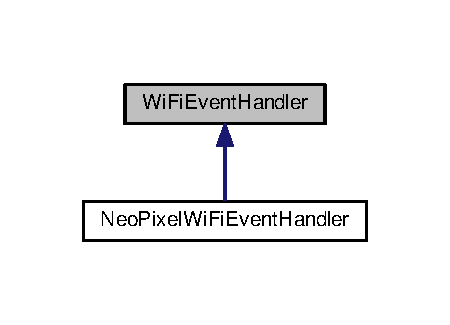
\includegraphics[width=216pt]{class_wi_fi_event_handler__inherit__graph}
\end{center}
\end{figure}
\subsection*{Public Member Functions}
\begin{DoxyCompactItemize}
\item 
system\+\_\+event\+\_\+cb\+\_\+t \hyperlink{class_wi_fi_event_handler_a9eeffe417501462c8a12a9e879a69444}{get\+Event\+Handler} ()
\item 
virtual esp\+\_\+err\+\_\+t {\bfseries ap\+Sta\+Connected} ()\hypertarget{class_wi_fi_event_handler_a4ee55ebb6efef5eaedf92659de6ba41d}{}\label{class_wi_fi_event_handler_a4ee55ebb6efef5eaedf92659de6ba41d}

\item 
virtual esp\+\_\+err\+\_\+t {\bfseries ap\+Sta\+Disconnected} ()\hypertarget{class_wi_fi_event_handler_a90051d0d6bf11854669b9eb2099c5371}{}\label{class_wi_fi_event_handler_a90051d0d6bf11854669b9eb2099c5371}

\item 
virtual esp\+\_\+err\+\_\+t {\bfseries ap\+Start} ()\hypertarget{class_wi_fi_event_handler_ad7f61897eeb4921461fd12c959b5b979}{}\label{class_wi_fi_event_handler_ad7f61897eeb4921461fd12c959b5b979}

\item 
virtual esp\+\_\+err\+\_\+t {\bfseries ap\+Stop} ()\hypertarget{class_wi_fi_event_handler_ae59d30f07785f4776ba348addde57d9e}{}\label{class_wi_fi_event_handler_ae59d30f07785f4776ba348addde57d9e}

\item 
virtual esp\+\_\+err\+\_\+t {\bfseries sta\+Connected} ()\hypertarget{class_wi_fi_event_handler_af12640a72f3563a1d0ba6abf15fd3621}{}\label{class_wi_fi_event_handler_af12640a72f3563a1d0ba6abf15fd3621}

\item 
virtual esp\+\_\+err\+\_\+t {\bfseries sta\+Disconnected} ()\hypertarget{class_wi_fi_event_handler_ab812cd56db587d6fd346257a1d33d53e}{}\label{class_wi_fi_event_handler_ab812cd56db587d6fd346257a1d33d53e}

\item 
virtual esp\+\_\+err\+\_\+t \hyperlink{class_wi_fi_event_handler_ab01ad1cdc445bb2107125ec89a71886d}{sta\+Got\+Ip} (system\+\_\+event\+\_\+sta\+\_\+got\+\_\+ip\+\_\+t event\+\_\+sta\+\_\+got\+\_\+ip)
\item 
virtual esp\+\_\+err\+\_\+t {\bfseries sta\+Start} ()\hypertarget{class_wi_fi_event_handler_a42497c852ceb28651432e887a7c5405d}{}\label{class_wi_fi_event_handler_a42497c852ceb28651432e887a7c5405d}

\item 
virtual esp\+\_\+err\+\_\+t {\bfseries sta\+Stop} ()\hypertarget{class_wi_fi_event_handler_a1b3311f207915c563e37da0a7ae901ac}{}\label{class_wi_fi_event_handler_a1b3311f207915c563e37da0a7ae901ac}

\item 
virtual esp\+\_\+err\+\_\+t {\bfseries wifi\+Ready} ()\hypertarget{class_wi_fi_event_handler_a52ccc311c3ddd1c1da162da356bee2e8}{}\label{class_wi_fi_event_handler_a52ccc311c3ddd1c1da162da356bee2e8}

\item 
\hyperlink{class_wi_fi_event_handler}{Wi\+Fi\+Event\+Handler} $\ast$ \hyperlink{class_wi_fi_event_handler_a0b24b1ee868a02ec650205f79b0b04c4}{get\+Next\+Handler} ()
\item 
void \hyperlink{class_wi_fi_event_handler_afee45469141ee1351e06609ad0050133}{set\+Next\+Handler} (\hyperlink{class_wi_fi_event_handler}{Wi\+Fi\+Event\+Handler} $\ast$next\+Handler)
\end{DoxyCompactItemize}


\subsection{Detailed Description}
Wi\+Fi state event handler. 

Here is an example class that implements all the virtual functions that can be called for events\+:


\begin{DoxyCode}
MyHandler::MyHandler() \{
\}

MyHandler::~MyHandler() \{
\}

esp\_err\_t MyHandler::apStart() \{
  \textcolor{keywordflow}{return} ESP\_OK;
\}

esp\_err\_t MyHandler::staConnected() \{
  \textcolor{keywordflow}{return} ESP\_OK;
\}

esp\_err\_t MyHandler::staDisconnected() \{
  \textcolor{keywordflow}{return} ESP\_OK;
\}

esp\_err\_t MyHandler::staStart() \{
  \textcolor{keywordflow}{return} ESP\_OK;
\}

esp\_err\_t MyHandler::staGotIp(system\_event\_sta\_got\_ip\_t event\_sta\_got\_ip) \{
  \textcolor{keywordflow}{return} ESP\_OK;
\}

esp\_err\_t MyHandler::wifiReady() \{
  \textcolor{keywordflow}{return} ESP\_OK;
\}
\end{DoxyCode}
 

\subsection{Member Function Documentation}
\index{Wi\+Fi\+Event\+Handler@{Wi\+Fi\+Event\+Handler}!get\+Event\+Handler@{get\+Event\+Handler}}
\index{get\+Event\+Handler@{get\+Event\+Handler}!Wi\+Fi\+Event\+Handler@{Wi\+Fi\+Event\+Handler}}
\subsubsection[{\texorpdfstring{get\+Event\+Handler()}{getEventHandler()}}]{\setlength{\rightskip}{0pt plus 5cm}system\+\_\+event\+\_\+cb\+\_\+t Wi\+Fi\+Event\+Handler\+::get\+Event\+Handler (
\begin{DoxyParamCaption}
{}
\end{DoxyParamCaption}
)}\hypertarget{class_wi_fi_event_handler_a9eeffe417501462c8a12a9e879a69444}{}\label{class_wi_fi_event_handler_a9eeffe417501462c8a12a9e879a69444}
Retrieve the event handler function to be passed to the E\+S\+P-\/\+I\+DF event handler system. \begin{DoxyReturn}{Returns}
The event handler function. 
\end{DoxyReturn}
\index{Wi\+Fi\+Event\+Handler@{Wi\+Fi\+Event\+Handler}!get\+Next\+Handler@{get\+Next\+Handler}}
\index{get\+Next\+Handler@{get\+Next\+Handler}!Wi\+Fi\+Event\+Handler@{Wi\+Fi\+Event\+Handler}}
\subsubsection[{\texorpdfstring{get\+Next\+Handler()}{getNextHandler()}}]{\setlength{\rightskip}{0pt plus 5cm}{\bf Wi\+Fi\+Event\+Handler}$\ast$ Wi\+Fi\+Event\+Handler\+::get\+Next\+Handler (
\begin{DoxyParamCaption}
{}
\end{DoxyParamCaption}
)\hspace{0.3cm}{\ttfamily [inline]}}\hypertarget{class_wi_fi_event_handler_a0b24b1ee868a02ec650205f79b0b04c4}{}\label{class_wi_fi_event_handler_a0b24b1ee868a02ec650205f79b0b04c4}
Get the next Wi\+Fi event handler in the chain, if there is one. \begin{DoxyReturn}{Returns}
The next Wi\+Fi event handler in the chain or nullptr if there is none. 
\end{DoxyReturn}
\index{Wi\+Fi\+Event\+Handler@{Wi\+Fi\+Event\+Handler}!set\+Next\+Handler@{set\+Next\+Handler}}
\index{set\+Next\+Handler@{set\+Next\+Handler}!Wi\+Fi\+Event\+Handler@{Wi\+Fi\+Event\+Handler}}
\subsubsection[{\texorpdfstring{set\+Next\+Handler(\+Wi\+Fi\+Event\+Handler $\ast$next\+Handler)}{setNextHandler(WiFiEventHandler *nextHandler)}}]{\setlength{\rightskip}{0pt plus 5cm}void Wi\+Fi\+Event\+Handler\+::set\+Next\+Handler (
\begin{DoxyParamCaption}
\item[{{\bf Wi\+Fi\+Event\+Handler} $\ast$}]{next\+Handler}
\end{DoxyParamCaption}
)\hspace{0.3cm}{\ttfamily [inline]}}\hypertarget{class_wi_fi_event_handler_afee45469141ee1351e06609ad0050133}{}\label{class_wi_fi_event_handler_afee45469141ee1351e06609ad0050133}
Set the next Wi\+Fi event handler in the chain. 
\begin{DoxyParams}[1]{Parameters}
\mbox{\tt in}  & {\em next\+Handler} & The next Wi\+Fi event handler in the chain. \\
\hline
\end{DoxyParams}
\index{Wi\+Fi\+Event\+Handler@{Wi\+Fi\+Event\+Handler}!sta\+Got\+Ip@{sta\+Got\+Ip}}
\index{sta\+Got\+Ip@{sta\+Got\+Ip}!Wi\+Fi\+Event\+Handler@{Wi\+Fi\+Event\+Handler}}
\subsubsection[{\texorpdfstring{sta\+Got\+Ip(system\+\_\+event\+\_\+sta\+\_\+got\+\_\+ip\+\_\+t event\+\_\+sta\+\_\+got\+\_\+ip)}{staGotIp(system_event_sta_got_ip_t event_sta_got_ip)}}]{\setlength{\rightskip}{0pt plus 5cm}esp\+\_\+err\+\_\+t Wi\+Fi\+Event\+Handler\+::sta\+Got\+Ip (
\begin{DoxyParamCaption}
\item[{system\+\_\+event\+\_\+sta\+\_\+got\+\_\+ip\+\_\+t}]{event\+\_\+sta\+\_\+got\+\_\+ip}
\end{DoxyParamCaption}
)\hspace{0.3cm}{\ttfamily [virtual]}}\hypertarget{class_wi_fi_event_handler_ab01ad1cdc445bb2107125ec89a71886d}{}\label{class_wi_fi_event_handler_ab01ad1cdc445bb2107125ec89a71886d}
Handle having received/assigned an IP address when we are a station. \begin{DoxyReturn}{Returns}
An indication of whether or not we processed the event successfully. 
\end{DoxyReturn}


Reimplemented in \hyperlink{class_neo_pixel_wi_fi_event_handler_a3e9dffc7ccc2fab6e202695e53e3283a}{Neo\+Pixel\+Wi\+Fi\+Event\+Handler}.



The documentation for this class was generated from the following files\+:\begin{DoxyCompactItemize}
\item 
Wi\+Fi\+Event\+Handler.\+h\item 
Wi\+Fi\+Event\+Handler.\+cpp\end{DoxyCompactItemize}

\hypertarget{class_w_s2812}{}\section{W\+S2812 Class Reference}
\label{class_w_s2812}\index{W\+S2812@{W\+S2812}}


Driver for W\+S2812/\+Neo\+Pixel data.  




{\ttfamily \#include $<$W\+S2812.\+h$>$}

\subsection*{Public Member Functions}
\begin{DoxyCompactItemize}
\item 
\hyperlink{class_w_s2812_a873e567f57a612a0e408b5bb310d9024}{W\+S2812} (gpio\+\_\+num\+\_\+t gpio\+Num, uint16\+\_\+t pixel\+Count, int channel=R\+M\+T\+\_\+\+C\+H\+A\+N\+N\+E\+L\+\_\+0)
\begin{DoxyCompactList}\small\item\em Construct a wrapper for the pixels. \end{DoxyCompactList}\item 
void \hyperlink{class_w_s2812_ad03797836617dccf530cb7c6423c03fe}{show} ()
\begin{DoxyCompactList}\small\item\em Show the current Neopixel data. \end{DoxyCompactList}\item 
void \hyperlink{class_w_s2812_a7a68e53534f4b1f68e447621caf0e2e6}{set\+Color\+Order} (char $\ast$order)
\begin{DoxyCompactList}\small\item\em Set the color order of data sent to the L\+E\+Ds. \end{DoxyCompactList}\item 
void \hyperlink{class_w_s2812_a60025d23e7fc21c3ce8c1f02bd50bf86}{set\+Pixel} (uint16\+\_\+t index, uint8\+\_\+t red, uint8\+\_\+t green, uint8\+\_\+t blue)
\begin{DoxyCompactList}\small\item\em Set the given pixel to the specified color. \end{DoxyCompactList}\item 
void \hyperlink{class_w_s2812_a2f37824dbf4730986d4ebde58c25a48d}{set\+Pixel} (uint16\+\_\+t index, \hyperlink{structpixel__t}{pixel\+\_\+t} pixel)
\begin{DoxyCompactList}\small\item\em Set the given pixel to the specified color. \end{DoxyCompactList}\item 
void \hyperlink{class_w_s2812_a65924d977bab621786b01a09c91456f6}{set\+Pixel} (uint16\+\_\+t index, uint32\+\_\+t pixel)
\begin{DoxyCompactList}\small\item\em Set the given pixel to the specified color. \end{DoxyCompactList}\item 
void \hyperlink{class_w_s2812_aceeaba644d2cc545b84d2807732b6461}{clear} ()
\begin{DoxyCompactList}\small\item\em Clear all the pixel colors. \end{DoxyCompactList}\item 
virtual \hyperlink{class_w_s2812_a58973dedd9cbc5c3fd3397f07f9a720f}{$\sim$\+W\+S2812} ()\hypertarget{class_w_s2812_a58973dedd9cbc5c3fd3397f07f9a720f}{}\label{class_w_s2812_a58973dedd9cbc5c3fd3397f07f9a720f}

\begin{DoxyCompactList}\small\item\em Class instance destructor. \end{DoxyCompactList}\end{DoxyCompactItemize}


\subsection{Detailed Description}
Driver for W\+S2812/\+Neo\+Pixel data. 

Neo\+Pixels or W\+S2812s are L\+ED devices that can illuminate in arbitrary colors with 8 bits of data for each of the red, green and blue channels. These devices can be daisy chained together to produce a string of L\+E\+Ds. If we call each L\+ED instance a pixel, then when we want to set the value of a string of pixels, we need to supply the data for all the pixels. This class encapsulates setting the color value for an individual pixel within the string and, once you have set up all the desired colors, you can then set all the pixels in a \hyperlink{class_w_s2812_ad03797836617dccf530cb7c6423c03fe}{show()} operation. The class hides from you the underlying details needed to drive the devices.


\begin{DoxyCode}
\hyperlink{class_w_s2812}{WS2812} ws2812 = \hyperlink{class_w_s2812_a873e567f57a612a0e408b5bb310d9024}{WS2812}(
  16, \textcolor{comment}{// Pin}
  8   \textcolor{comment}{// Pixel count}
);
ws2812.\hyperlink{class_w_s2812_a60025d23e7fc21c3ce8c1f02bd50bf86}{setPixel}(0, 128, 0, 0);
ws2812.\hyperlink{class_w_s2812_ad03797836617dccf530cb7c6423c03fe}{show}();
\end{DoxyCode}
 

\subsection{Constructor \& Destructor Documentation}
\index{W\+S2812@{W\+S2812}!W\+S2812@{W\+S2812}}
\index{W\+S2812@{W\+S2812}!W\+S2812@{W\+S2812}}
\subsubsection[{\texorpdfstring{W\+S2812(gpio\+\_\+num\+\_\+t gpio\+Num, uint16\+\_\+t pixel\+Count, int channel=\+R\+M\+T\+\_\+\+C\+H\+A\+N\+N\+E\+L\+\_\+0)}{WS2812(gpio_num_t gpioNum, uint16_t pixelCount, int channel=RMT_CHANNEL_0)}}]{\setlength{\rightskip}{0pt plus 5cm}W\+S2812\+::\+W\+S2812 (
\begin{DoxyParamCaption}
\item[{gpio\+\_\+num\+\_\+t}]{din\+Pin, }
\item[{uint16\+\_\+t}]{pixel\+Count, }
\item[{int}]{channel = {\ttfamily RMT\+\_\+CHANNEL\+\_\+0}}
\end{DoxyParamCaption}
)}\hypertarget{class_w_s2812_a873e567f57a612a0e408b5bb310d9024}{}\label{class_w_s2812_a873e567f57a612a0e408b5bb310d9024}


Construct a wrapper for the pixels. 

In order to drive the Neo\+Pixels we need to supply some basic information. This includes the \hyperlink{class_g_p_i_o}{G\+P\+IO} pin that is connected to the data-\/in (D\+IN) of the devices. Since we also want to be able to drive a string of pixels, we need to tell the class how many pixels are present in the string.


\begin{DoxyParams}[1]{Parameters}
\mbox{\tt in}  & {\em gpio\+Num} & The \hyperlink{class_g_p_i_o}{G\+P\+IO} pin used to drive the data. \\
\hline
\mbox{\tt in}  & {\em pixel\+Count} & The number of pixels in the strand. \\
\hline
\mbox{\tt in}  & {\em channel} & The \hyperlink{class_r_m_t}{R\+MT} channel to use. Defaults to R\+M\+T\+\_\+\+C\+H\+A\+N\+N\+E\+L\+\_\+0. \\
\hline
\end{DoxyParams}


\subsection{Member Function Documentation}
\index{W\+S2812@{W\+S2812}!clear@{clear}}
\index{clear@{clear}!W\+S2812@{W\+S2812}}
\subsubsection[{\texorpdfstring{clear()}{clear()}}]{\setlength{\rightskip}{0pt plus 5cm}void W\+S2812\+::clear (
\begin{DoxyParamCaption}
{}
\end{DoxyParamCaption}
)}\hypertarget{class_w_s2812_aceeaba644d2cc545b84d2807732b6461}{}\label{class_w_s2812_aceeaba644d2cc545b84d2807732b6461}


Clear all the pixel colors. 

This sets all the pixels to off which is no brightness for all of the color channels. The L\+E\+Ds are not actually updated until a call to \hyperlink{class_w_s2812_ad03797836617dccf530cb7c6423c03fe}{show()}. \index{W\+S2812@{W\+S2812}!set\+Color\+Order@{set\+Color\+Order}}
\index{set\+Color\+Order@{set\+Color\+Order}!W\+S2812@{W\+S2812}}
\subsubsection[{\texorpdfstring{set\+Color\+Order(char $\ast$order)}{setColorOrder(char *order)}}]{\setlength{\rightskip}{0pt plus 5cm}void W\+S2812\+::set\+Color\+Order (
\begin{DoxyParamCaption}
\item[{char $\ast$}]{color\+Order}
\end{DoxyParamCaption}
)}\hypertarget{class_w_s2812_a7a68e53534f4b1f68e447621caf0e2e6}{}\label{class_w_s2812_a7a68e53534f4b1f68e447621caf0e2e6}


Set the color order of data sent to the L\+E\+Ds. 

Data is sent to the W\+S2812s in a serial fashion. There are 8 bits of data for each of the three channel colors (red, green and blue). The \hyperlink{class_w_s2812}{W\+S2812} L\+E\+Ds typically expect the data to arrive in the order of \char`\"{}green\char`\"{} then \char`\"{}red\char`\"{} then \char`\"{}blue\char`\"{}. However, this has been found to vary between some models and manufacturers. What this means is that some want \char`\"{}red\char`\"{}, \char`\"{}green\char`\"{}, \char`\"{}blue\char`\"{} and still others have their own orders. This function can be called to override the default ordering of \char`\"{}\+G\+R\+B\char`\"{}. We can specify an alternate order by supply an alternate three character string made up of \textquotesingle{}R\textquotesingle{}, \textquotesingle{}G\textquotesingle{} and \textquotesingle{}B\textquotesingle{} for example \char`\"{}\+R\+G\+B\char`\"{}. \index{W\+S2812@{W\+S2812}!set\+Pixel@{set\+Pixel}}
\index{set\+Pixel@{set\+Pixel}!W\+S2812@{W\+S2812}}
\subsubsection[{\texorpdfstring{set\+Pixel(uint16\+\_\+t index, uint8\+\_\+t red, uint8\+\_\+t green, uint8\+\_\+t blue)}{setPixel(uint16_t index, uint8_t red, uint8_t green, uint8_t blue)}}]{\setlength{\rightskip}{0pt plus 5cm}void W\+S2812\+::set\+Pixel (
\begin{DoxyParamCaption}
\item[{uint16\+\_\+t}]{index, }
\item[{uint8\+\_\+t}]{red, }
\item[{uint8\+\_\+t}]{green, }
\item[{uint8\+\_\+t}]{blue}
\end{DoxyParamCaption}
)}\hypertarget{class_w_s2812_a60025d23e7fc21c3ce8c1f02bd50bf86}{}\label{class_w_s2812_a60025d23e7fc21c3ce8c1f02bd50bf86}


Set the given pixel to the specified color. 

The L\+E\+Ds are not actually updated until a call to \hyperlink{class_w_s2812_ad03797836617dccf530cb7c6423c03fe}{show()}.


\begin{DoxyParams}[1]{Parameters}
\mbox{\tt in}  & {\em index} & The pixel that is to have its color set. \\
\hline
\mbox{\tt in}  & {\em red} & The amount of red in the pixel. \\
\hline
\mbox{\tt in}  & {\em green} & The amount of green in the pixel. \\
\hline
\mbox{\tt in}  & {\em blue} & The amount of blue in the pixel. \\
\hline
\end{DoxyParams}
\index{W\+S2812@{W\+S2812}!set\+Pixel@{set\+Pixel}}
\index{set\+Pixel@{set\+Pixel}!W\+S2812@{W\+S2812}}
\subsubsection[{\texorpdfstring{set\+Pixel(uint16\+\_\+t index, pixel\+\_\+t pixel)}{setPixel(uint16_t index, pixel_t pixel)}}]{\setlength{\rightskip}{0pt plus 5cm}void W\+S2812\+::set\+Pixel (
\begin{DoxyParamCaption}
\item[{uint16\+\_\+t}]{index, }
\item[{{\bf pixel\+\_\+t}}]{pixel}
\end{DoxyParamCaption}
)}\hypertarget{class_w_s2812_a2f37824dbf4730986d4ebde58c25a48d}{}\label{class_w_s2812_a2f37824dbf4730986d4ebde58c25a48d}


Set the given pixel to the specified color. 

The L\+E\+Ds are not actually updated until a call to \hyperlink{class_w_s2812_ad03797836617dccf530cb7c6423c03fe}{show()}.


\begin{DoxyParams}[1]{Parameters}
\mbox{\tt in}  & {\em index} & The pixel that is to have its color set. \\
\hline
\mbox{\tt in}  & {\em pixel} & The color value of the pixel. \\
\hline
\end{DoxyParams}
\index{W\+S2812@{W\+S2812}!set\+Pixel@{set\+Pixel}}
\index{set\+Pixel@{set\+Pixel}!W\+S2812@{W\+S2812}}
\subsubsection[{\texorpdfstring{set\+Pixel(uint16\+\_\+t index, uint32\+\_\+t pixel)}{setPixel(uint16_t index, uint32_t pixel)}}]{\setlength{\rightskip}{0pt plus 5cm}void W\+S2812\+::set\+Pixel (
\begin{DoxyParamCaption}
\item[{uint16\+\_\+t}]{index, }
\item[{uint32\+\_\+t}]{pixel}
\end{DoxyParamCaption}
)}\hypertarget{class_w_s2812_a65924d977bab621786b01a09c91456f6}{}\label{class_w_s2812_a65924d977bab621786b01a09c91456f6}


Set the given pixel to the specified color. 

The L\+E\+Ds are not actually updated until a call to \hyperlink{class_w_s2812_ad03797836617dccf530cb7c6423c03fe}{show()}.


\begin{DoxyParams}[1]{Parameters}
\mbox{\tt in}  & {\em index} & The pixel that is to have its color set. \\
\hline
\mbox{\tt in}  & {\em pixel} & The color value of the pixel. \\
\hline
\end{DoxyParams}
\index{W\+S2812@{W\+S2812}!show@{show}}
\index{show@{show}!W\+S2812@{W\+S2812}}
\subsubsection[{\texorpdfstring{show()}{show()}}]{\setlength{\rightskip}{0pt plus 5cm}void W\+S2812\+::show (
\begin{DoxyParamCaption}
{}
\end{DoxyParamCaption}
)}\hypertarget{class_w_s2812_ad03797836617dccf530cb7c6423c03fe}{}\label{class_w_s2812_ad03797836617dccf530cb7c6423c03fe}


Show the current Neopixel data. 

Drive the L\+E\+Ds with the values that were previously set. 

The documentation for this class was generated from the following files\+:\begin{DoxyCompactItemize}
\item 
W\+S2812.\+h\item 
W\+S2812.\+cpp\end{DoxyCompactItemize}

%--- End generated contents ---

% Index
\backmatter
\newpage
\phantomsection
\clearemptydoublepage
\addcontentsline{toc}{chapter}{Index}
\printindex

\end{document}
